\documentclass[10pt, conference,compsoc]{IEEEtran}
% Some/most Computer Society conferences require the compsoc mode option,
% but others may want the standard conference format.
%
% If IEEEtran.cls has not been installed into the LaTeX system files,
% manually specify the path to it like:
% \documentclass[conference,compsoc]{../sty/IEEEtran}


% Some very useful LaTeX packages include:
% (uncomment the ones you want to load)


% *** MISC UTILITY PACKAGES ***
%
\usepackage{ifpdf}
% Heiko Oberdiek's ifpdf.sty is very useful if you need conditional
% compilation based on whether the output is pdf or dvi.
% usage:
% \ifpdf
%   % pdf code
% \else
%   % dvi code
% \fi
% The latest version of ifpdf.sty can be obtained from:
% http://www.ctan.org/pkg/ifpdf
% Also, note that IEEEtran.cls V1.7 and later provides a builtin
% \ifCLASSINFOpdf conditional that works the same way.
% When switching from latex to pdflatex and vice-versa, the compiler may
% have to be run twice to clear warning/error messages.


% *** CITATION PACKAGES ***
%
\ifCLASSOPTIONcompsoc
  % IEEE Computer Society needs nocompress option
  % requires cite.sty v4.0 or later (November 2003)
  \usepackage[nocompress]{cite}
\else
  % normal IEEE
  \usepackage{cite}
\fi

% *** GRAPHICS RELATED PACKAGES ***
%
\ifCLASSINFOpdf
        \usepackage[pdftex]{graphicx}
        % declare the path(s) where your graphic files are
        \graphicspath{{figures/}}
        % and their extensions so you won't have to specify these with
        % every instance of \includegraphics
        \DeclareGraphicsExtensions{.pdf,.jpeg,.png}
\else
        % or other class option (dvipsone, dvipdf, if not using dvips). graphicx
        % will default to the driver specified in the system graphics.cfg if no
        % driver is specified.
\usepackage[dvips]{graphicx}
        % declare the path(s) where your graphic files are
        \graphicspath{{figures/}}
        % and their extensions so you won't have to specify these with
        % every instance of \includegraphics
        \DeclareGraphicsExtensions{.eps}
\fi


% *** MATH PACKAGES ***
%
\usepackage{amsmath}
\usepackage{cuted}

\newcommand\numberthis{\addtocounter{equation}{1}\tag{\theequation}}

% *** SPECIALIZED LIST PACKAGES ***
%
\usepackage{algorithm}
\usepackage{algpseudocode}
\usepackage{booktabs}
\usepackage{enumitem}
\usepackage{mathrsfs}

% *** ALIGNMENT PACKAGES ***
%
\usepackage{array}

% *** SUBFIGURE PACKAGES ***
\ifCLASSOPTIONcompsoc
        \usepackage[caption=false,font=footnotesize,labelfont=sf,textfont=sf]{subfig}
\else
        \usepackage[caption=false,font=footnotesize]{subfig}
\fi


%*******to add comment tag***********
\usepackage{verbatim}
\usepackage{soul}
\usepackage{xcolor}
\newcommand{\TODO}[1]{\hl{TODO: #1}}
\newcommand{\NOTE}[1]{\hl {NOTE: #1}}
% \newcommand{\changed}[1]{\textcolor{red}{#1}}


% *** PDF, URL AND HYPERLINK PACKAGES ***
%
\usepackage{url}


% correct bad hyphenation here
\hyphenation{op-tical net-works semi-conduc-tor}

\addtolength{\jot}{0.4em}


\newcommand{\equref}[1]{(\ref{#1})}

\begin{document}
%
% paper title
% Titles are generally capitalized except for words such as a, an, and, as,
% at, but, by, for, in, nor, of, on, or, the, to and up, which are usually
% not capitalized unless they are the first or last word of the title.
% Linebreaks \\ can be used within to get better formatting as desired.
% Do not put math or special symbols in the title.
\title{Cerberus: a 3-Phase Burst Buffer Aware Batch Scheduler for HPC Systems}


% author names and affiliations
% use a multiple column layout for up to three different
% affiliations
\author{\IEEEauthorblockN{Jiaqi Yan and Xu Yang and Xin Wang}
\IEEEauthorblockA{Department of Computer Science\\
Illinois Institute of Technology\\
10 West 31st Street\\
Chicago, IL, United States\\
Email: \{jyan31, xyang56, xwang925\}@hawk.iit.edu
}
\and
\IEEEauthorblockN{Dong Jin and Zhiling Lan}
\IEEEauthorblockA{Department of Computer Science\\
Illinois Institute of Technology\\
10 West 31st Street\\
Chicago, IL, United States\\
Email: \{dong.jin, lan\}@iit.edu
}
}


% use for special paper notices
%\IEEEspecialpapernotice{(Invited Paper)}


\maketitle

\begin{abstract}
Burst buffer drastically improves the performance of computational applications by providing high perceived I/O bandwidth.
However, traditional batch schedulers have barely embraced the full potential of burst buffer technology in practice. 
%either barely knows BB's existence or cannot fully utilize them in practice.
In this paper, we model the execution of scientific applications
that generate tens of TB of data on a supercomputer equipped with burst buffer.
We characterize the lifetime of generic applications into three phases:
\textit{stage-in}, \textit{running}, and \textit{stage-out}.
We develop a novel burst-buffer-aware batch scheduler \textit{Cerberus} to 
manage resource allocation in different phases.
In both stage-in and stage-out phases, Cerberus
allocates the burst buffer resources to achieve the maximum data transfer throughput
between burst buffer and the external storage system.
In the running phase, Cerberus maximizes the predefined objectives of job scheduling.
We evaluate our design through extensive event driven simulations. 
Our preliminary results demonstrate that
1) compared to non-burst-buffer systems, Cerberus accelerates the job execution, reduces the job response time, and improves average system throughput by 192\%;
2) three-phase based Cerberus extra boosts the average system throughput by 62\% comparing to traditional static burst-buffer-aware batch scheduler.
\end{abstract}

\IEEEpeerreviewmaketitle

\section{Introduction}

In the field of high performance computing (HPC), 
system performance is no longer throttled only by computation capability,
but also by the ever-increasing I/O gap
between computational resources and disk-based storage technologies.
For example, on the early-state Trinity system~\cite{TrinitySystem}, the I/O nodes between
the compute nodes and the external storage can deliver transfer speed at 810 GB/s,
which is still far from the target of 60 TB/s for the exascale computers\cite{Shalf:HPCCS:2010}.
The gap is critical because scientific applications typically exhibit
``bursty" I/O patterns,
resulting from application's defensive I/O strategy
and the need  for subsequent data processing\cite{Carns:MSST:2011, Kim:PDSW:2010, Latham:CSD:2012, Naik:ICPPW:2009, Dennis:CUG:2009}. 
When multiple applications attempt to access the storage system simultaneously, 
it is easy to saturate
the I/O bandwidth, leading to severe performance degradation.


%3. Very high level intro to burst buffer
Extensive research have been conducted to improve I/O performance on HPC systems from
both hardware and software layers.
We have witnessed a tremendously growing use of flash memory based storage in recent years.
Recently, burst buffer (i.e., a solid state disk based or flash based cache tier)
is proposed to absorb and spread out
the ``bursty" application I/O patterns\cite{Bent:HBP:2011, Grider:EXA:2010}.
% This new cache tier is capable of absorbing and spreading out 
% the ``bursty" application I/O pattern\cite{Bent:HBP:2011, Grider:EXA:2010}.
Studies have demonstrated that the perceived I/O
bandwidth can be significantly improved on burst-buffer-enabled systems\cite{Liu:MSST:2012}.
As such, HPC users are encouraged to explicitly request burst buffer resources at job submission 
on burst-buffer-enabled systems\cite{apex-workflow}.

%4. Our work, a new batch scheduler
In this paper, we propose \textit{Cerberus}\footnote{In Greek mythology,
Cerberus is a monstrous three-headed dog (three-phase scheduler),
who guards the gate of the underworld to the earth (HPC system),
preventing the dead (jobs) from leaving (running).},
a novel batch scheduler for HPC systems equipped with burst buffer. 
We propose a three-phase job model.
%based on the critical use cases of burst buffer, including
%application checkpoint restart and staging in/out data. 
The lifetime of a user job is divided into three logic phases:
\textit{stage in}, \textit{running}, and \textit{stage-out}.
Burst buffer is used for different purposes in these phases.
Unlike existing batch schedulers that make scheduling decision for each job upon its submission,
Cerberus participates in all of the three phases.
By dividing the lifetime of user jobs into three phases,
Cerberus adopts different optimization strategies to 
make scheduling decision based on job requirement at each phase.
We conduct a series of event driven simulations to evaluate our design. 
As shown later on,
the preliminary results demonstrate that the three-phase design of Cerberus 
not only boosts system responsiveness, but also improves job performance. 
Specifically,
Cerberus accelerates job execution, reduces job response time 
and improves the average system throughput.
Put together, we make three key contributions in this work:
\begin{enumerate}
        \item    We propose a three-phase job model (i.e., stage-in, running, and stage-out)
                to facilitate job scheduling in a fine granularity.
        \item    We present Cerberus, a three-phase burst buffer aware scheduler
                for HPC systems equipped with burst buffer.
                Our design consists of several key optimization strategies for
                improving the performance of user jobs throughout different job phases.
        \item    We develop an event driven simulator called BBSim
                for simulating and evaluating Cerberus on a burst buffer enabled Blue Gene system
                using authentic job trace. The simulator is open source and
                freely available to the community.
\end{enumerate}


In the remainder of this paper, Section 2 presents background and 
how existing batch scheduler handle burst buffer on HPC systems.
Section~\ref{Sec:Model} elaborates our three-phase job model.
Section~\ref{Sec:Scheduler} describes the design of Cerberus.
Section~\ref{Sec:Simulation} describes the design of BBsim, the event driven scheduling simulator.
Section~\ref{Sec:Experiments} evaluates Cerberus by comparing it with various alternatives.
Section~\ref{Sec:Conclusion} concludes this paper.



\section{Background and Existing Works}
\label{Sec:Background}

\begin{figure*}[h]
\centering
\subfloat[Naive Burst-Buffer Aware Scheduler, e.g. SLURM] {
        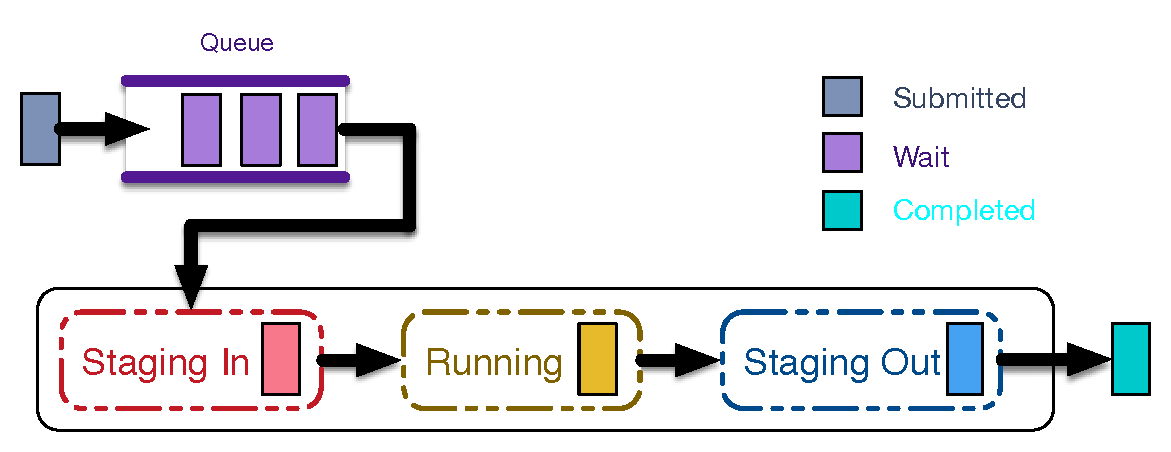
\includegraphics[width=3.1in]{SlurmQueue}
        \label{Fig:SlurmQueue}
}
\subfloat[Job Movement in Cerberus's Multiple Queues] {
        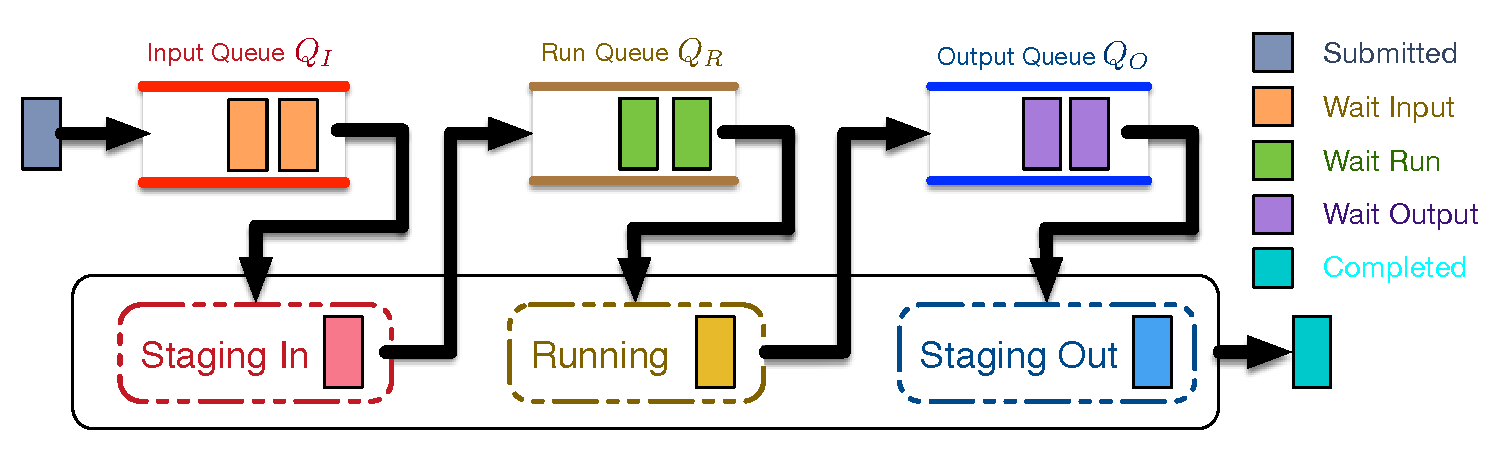
\includegraphics[width=3.7in]{CerberusQueues}
        \label{Fig:CerberusQueues}
}
\caption{Architecture Comparison: Single-Queue Adopted by Existing Batch Scheduler v.s. Multiple-Queue Used by Cerberus}
\label{Fig:CompareSlurmCerbuers}
\end{figure*}

%1. The appear of burst buffer
Burst buffer enabled I/O architecture can help alleviate
the ever-increasing I/O pressure on HPC systems.
It debuts as a rescue by utilizing various new storage technologies,
such as non-volatile random-access memory (NVRAM) and solid state drive (SSD).
In practice, burst buffer suits up with DataWarp I/O accelerator\cite{DataWarp}.
Figure \ref{Fig:BBArchitecture} illustrates one burst-buffer-enabled architecture,
adopted by the Trinity System\cite{TrinitySystem}.
%The volume of data read/write may affect the architecture model of burst buffer.
In Trinity, the burst buffer node is composed of one I/O node and 2 PCIe SSD cards,
connected via 16 PCIe 3.0 interfaces.
Alternatively, many researchers have proposed to distribute burst buffer 
on multiple layers of the memory hierarchy\cite{Romanus:CORR:15}.
For example, they may be deployed on the local compute nodes, the board in the cabinet or the I/O nodes.
Burst buffer may also be utilized as the intermediate storage systems.

%2. Use cases of burst buffer
Regardless of the specific deployment, burst buffer nodes essentially augment
the I/O stack with an intermediate productive offloading layer, 
which can benefit jobs in multiple ways.
As discussed in some preliminary surveys\cite{apex-workflow} ,
jobs' latest checkpoints can be pre-staged
before the previous job terminates;
jobs can burst checkpoint to burst buffer
with extremely high speed (4.4-17.8 TB/s on Trinity);
upon termination, jobs are also able to drain off output data
asynchronously to the external parallel file system (PFS).
The bursty I/O operations can thus be aggregated and absorbed into the burst buffer,
which shifts the computation that follows the I/O bursts to an earlier moment,
while burst buffer nodes take charge of moving potentially TB-level volumes of data.
There are more use cases for burst buffer nodes.
Among them, \textit{data cache} is equally important to enhance the responsiveness
of applications by improving the perceived I/O bandwidth\cite{TrinitySystem}.
Shared object library or read-only configuration files are cached into burst buffer;
the list of input files specific to a group of compute nodes allocated to
a particular job are loaded into burst buffer prior to the execution.
Economical solid-state disks as a tier of burst buffer could also be used as
out-of-core complement to insufficient main memory\cite{Romanus:CORR:15},
or working place for data analysis (reductions, feature extraction compression etc.)
and visualization\cite{TrinitySystem}.

%3. Existing works SLURM as example
Given the critical role of burst buffer in future HPC systems,
users are encouraged to explicitly request this new resource for performance enhancement\cite{apex-workflow}.
Inspired by this requirement, it is necessary to holistically manage
the allocation of these precious I/O resources,
which naturally falls into the responsibilities of the batch scheduler.
Existing batch schedulers \cite{Moab, Cobalt, SlurmBBGuide, PBSonCRAY} have already claimed to
be aware of burst buffer, but in fact only deals with it in a naive way.

Figure~\ref{Fig:SlurmQueue} depicts the way existing burst-buffer-aware scheduler manages burst buffer.
For example, SLRUM developed a module that allocates burst buffer resources to the submitted user jobs.
The module extra considers if jobs' burst buffer requirements are meet when making scheduling decision.
With the pre-allocated burst buffer,
the I/O performance of user jobs indeed can be improved\cite{SlurmBBGuide}.
PBS supports burst buffer aware scheduling in similar way as SLURM:
jobs are only dispatched when both required burst buffer and computing resource are ready\cite{PBSonCRAY}.

%4. Problem of existing schedulers
However, there are three problems in such single-queueing framework.
First, even though job's lifetime is conceptionally divided into 3 phases
(e.g. staging in, running and staging out) by the existing batch schedulers like SLURM,
they are in fact just the running phase because scheduler cannot do anything once a job is kicked off.
Secondly, a dispatched job will keep taking up its computing nodes and burst buffer nodes during its entire execution duration.
One may argue that there are cases that a job only need burst buffer to do I/O operations,
and there are cases that job can release computing nodes as soon as computation results is buffered
in burst buffer.
Finally, burst buffer and computing nodes are allocated altogether
in the straightforward first-come, first-served manner, without doing any optimization.
In conclusion, the static burst-buffer-aware scheduling framework in Figure~\ref{Fig:SlurmQueue}
is far from fully exploiting the utilization of burst buffer.

%5. Brief intro about our works
This paper aims to bridge the two isolated fields of HPC architecture:
the novel burst buffer equipped HPC I/O subsystem and the
traditional batch job queueing subsystem.
The bridge builds upon a three-phase job model motivated by critical use cases of burst buffer.
In three-phase job model, users are encouraged to provide the burst buffer demand on submission
and the execution of job is modeled into stage-in, running and stage-out phases.
The user jobs will acquire different resources before entering each phase.
This three-phase job model enables our burst-buffer-aware scheduler, Cerberus,
to adopt the scheduling framework illustrated in Figure~\ref{Fig:CerberusQueues}.
Comparing with the existing batch scheduler like SLRUM and PBS,
our approach have the following advantages.

The most difference is that there are three queues in Cerberus.
In three phase model, job demands different kind of resources at each phase.
Cerberus can deal with different resource demand by holding jobs in particular phase in designated queue.
Besides, the finer granularity introduced by more queues can further exploit
both the computing nodes and burst buffer nodes.
When finishing each phases, job will release its acquired resources, making it possible
to be allocated to other jobs promptly.
For example, when the golden job finish running, it will release the burst buffer it used to
do checkpointing, which can be immediately available to jobs in any phases.
We also integrate queues in Cerberus with different optimization algorithms for the
objective of maximizing the resource utilization and the system throughput.

In the following sections, we demonstrate that when burst buffer is intelligently allocated
by our novel batch scheduler, the benefit is far beyond the higher hardware transfer bandwidth.
The job execution is expedited by having their bursty I/O requests absorbed by burst buffer.
The job waiting time is reduced via the contracted input/output stage in the scheduling pipeline.
To our best knowledge, this is the first attempt to holistically schedule jobs
running on the new burst-buffer-enabled HPC systems.



\section{Three-Phase Job Model}
\label{Sec:Model}

Before we give the details of our Cerberus design, 
in this section we describe our three-phase job model 
and the corresponding resource demand at each phase. 
 
\textbf{Stage-In}: After submitted to the HPC system,
         jobs need to prefetch data, such as configuration files, libraries and input data,
         from PFS to the burst buffer. We define this phase as \textit{stage-in}.
         The only resource needed by the job in this phase is the burst buffer.
         Users are encouraged to specify the amount of burst buffer required in the \textit{stage-in} phase.
         The job is ready to run when the data is prefetched into the burst buffer.
         If the input data is too large to read in as a whole, the \textit{stage-in} phase
         only tries to read in the first chunk of the data chunks which is sufficient for
         the application to start running in \textit{running} phase.
 
% \textbf{Running}: The scheduler allocates the job with the required
%          number of compute nodes and the amount of burst buffer. 
%          It then dispatches the job to the system for running.
%          This is defined as \textit{running} phase.
%          During the running phase, there could be frequent data exchange
%          between the compute nodes and the burst buffer.
%          For example, check-pointing could help to achieve high system fault tolerance.
%          There are also cases that input data is so large that it must be read in
%          chunks during job execution.

\textbf{Running}: The scheduler allocates the job with the required
         number of compute nodes and the amount of burst buffer. 
         It then dispatches the job to the system for running.
         This is defined as \textit{running} phase.
         During the running phase, there could be frequent data exchange
         between the compute nodes and the burst buffer. For exmaple,
         applications may periodically write 'checkpoints' of their execution. 
         There may also be in-situ/in-transit data analytics/visualization in large simulation applications.
         Some scientific workflows with coupled applications may also share, exchange and communicate
         large chunk of data during running phases\cite{Romanus:CORR:15}.  

\textbf{Stage-out}: When the job finishes computation and
         exits the \textit{running} phase, its output data need to be drained out
         to the external storage from the on-node memory. We define this as \textit{stage-out} phase.
         The job can release its compute nodes when the output data are staged out
         into the burst buffer at high speed. The burst buffer serves as an efficient
         I/O broker for the compute nodes and drains the output data to the external storage.


%While burst buffer has been utilized during all three phases,
%compute nodes are only required during the \textit{running} phase. 


%\subsection{Three-Phase Resource Demand Model}
% Users typically provide their resource demand for their jobs.
% This is the most important information scheduler could get from the users.
% Therefore, each job is associated with a demand vector in the form of $(c, rt)$
% where $c$ is the number of needed compute node in running phase,
% $rt$ is the requested runtime user can provide to help scheduler make decisions.
% To be burst buffer aware, demand vector should be augmented
% with fields defining user's request for burst buffer capacity.
% We consider two possible ways to do so.
% Corresponding to the typical usage cases of burst buffer,
% user may provide a \textit{burst buffer triple} in the form of $(bb\_in, bb\_run, bb\_out)$,
% where $bb\_in$ is the volume of burst buffer user predicted for staging in data files,
% $bb\_run$ is the volume of burst buffer user preferred for checkpointing during running,
% $bb\_out$ is the volume of burst buffer needed to hold the resulting output data.
% A job that providing demand vector augmented with
% burst buffer triple is called a \textit{3-phase modeled job}.
% Alternatively, a lazy user may just use the $\max\{bb\_in, bb\_run, bb\_out\}$ at every stage.
% %We do not make any assumption about $bb\_run$ and $bb\_out$
% %because it is nontrivial to predict them, both for system scheduler and application owner.
% We refer this augmentation as
% \textit{1-phase modeled jobs} thereafter.

%=========XY===============
Jobs are submitted to the system with the specified resource demand.
Each job is associated with a demand vector in the form of $(c, ert)$,
where $c$ is the number of needed compute nodes in the running phase,
$ert$ is the expected runtime.
In a burst-buffer-enabled system, the demand vector should be augmented
with fields defining user's requests on the burst buffer capacity.
We consider two possible ways that users provide the burst buffer demand.
For the users with accurate speculation about their job's burst buffer demand in each phase,
they may provide a \textit{burst buffer triple} in the form of $(bb\_in, bb\_run, bb\_out)$,
where $bb\_in$ is the volume of burst buffer in stage-in phase,
$bb\_run$ is the volume of the burst buffer in running phase, and
$bb\_out$ is the volume of the burst buffer for staging out the output data.
% A job that providing demand vector augmented with
% burst buffer triple is called a \textit{3-phase modeled job}.
We will show the benefits of providing the job burst buffer demand in the form of \textit{burst buffer triple} in Section~\ref{Sec:Experiments}.
Alternatively, a user may just use the $\max\{bb\_in, bb\_run, bb\_out\}$
as the job's burst buffer demand in the entire lifetime.
The three-phase job model does not assume any independence between three phases, which
discussed in more details in section~\ref{SubSec:Coordination}.
Table~\ref{Tab:Symbols} summarizes the meaning of symbols used in this paper.
% We refer this augmentation as
% \textit{1-phase modeled jobs} thereafter.

% The tightly coupling between processing cores and memory makes 3-phase model
% more complicated than it appears in terms of resource releasing.
% For a job at the stage-in phase, compute nodes is not allocated to it yet
% but that will not effect staging in data.
% When scheduler allocate compute nodes (coupled with memory) to a job,
% these nodes are exclusively used by this job.
% The first thing to do in running phase is fetching in data from burst buffer to memory,
% which is not available until compute nodes is allocated to job.
% We refer this sub-phase as \textit{fectch-in} phase.
% $bb\_in$ will be hold by job until \textit{fetch-in} phase finished.
% Even if the computation is done when job exit \textit{running phase},
% compute nodes cannot be released until job enters \textit{stage-out} phase 
% \textbf{and} output data are drained out to burst buffer from memory,
% referred as \textit{drain-out} phase.
% However, $bb\_run$ can be immediately reclaimed at the end of \textit{running phase}.
% Once \textit{drain-out} phase is done,
% compute nodes become available for jobs waiting to be run
% because staging output data out to I/O node is the business of burst buffer nodes,
% sometimes with the help from traditional I/O nodes.
% Burst buffer nodes used for caching output data can thus be put back for reuse
% when \textit{stage-out} phase, as well as the entire lifetime of job, concludes.



%The resource releasing for the 3-phase modeled jobs is nontrivial. 
%For a job at \textit{stage-in} phase, compute nodes is not allocated to it yet. 
%The job can stage in data from external storage to burst buffer without the involvement of compute nodes.
%When scheduler allocates compute nodes to the job, the job enters the \textit{running} phase 
%and starts to read the pre-fetched data from burst buffer into the main memory, 
%$bb\_in$ will be released after all the data are moved into main memory. 
%When the job finishes computation and exits \textit{running} phase, 
%$bb\_run$ are released while compute nodes are still hold by the job. 
%The compute nodes will be released after all the output data are moved into $bb\_out$ from main memory.
%The job at \textit{stage-out} phase only holds $bb\_out$ burst buffer. 
%Once all the output data are drained out to the external storage,  
%$bb\_out$ is released.


\begin{table}[h] 
        \renewcommand{\arraystretch}{1.3}
        \caption{Summary of Symbols}
        \label{Tab:Symbols}
        \centering
        \begin{tabular}{l|l}
                \hline
                $CN$ & number of total compute nodes \\
                $BB$ & amount of total burst buffer nodes \\
                $CN_{available}$ & number of available compute nodes \\
                $BB_{available}$ & amount of available burst buffer nodes \\
                $c_i$ & compute node demand of $job_i$ \\
                $bb\_in_i$ & burst buffer demand of $job_i$ at \textit{stage-in} phase \\
                $bb\_run_i$ & burst buffer demand of $job_i$ at \textit{running} phase \\
                $bb\_out_i$ & burst buffer demand of $job_i$ at \textit{stage-out} phase \\
                $rt_i$ & running time of $job_i$ recorded in the log trace \\
                $ert_i$ & estimated or expected running time of $job_i$ \\
                $Q_I, Q_R, Q_O$ & queues for \textit{stage-in, running, stage-out} phases \\
                $J_{Q_I}, J_{Q_R}, J_{Q_O}$ & set of jobs in corresponding queues \\
                $\mathcal{J}_{Q_I}, \mathcal{J}_{Q_R}, \mathcal{J}_{Q_O}$ & selected jobs from the corresponding queues\\
                $p_i$ & profit of $job_i \in J_{Q_R}$ \\
                $dp(\cdot)$ & memoization used in dynamic programming \\
                \hline
        \end{tabular}
\end{table}



\section{Design of Cerberus}
\label{Sec:Scheduler}

\begin{figure}[htp]
\centering
        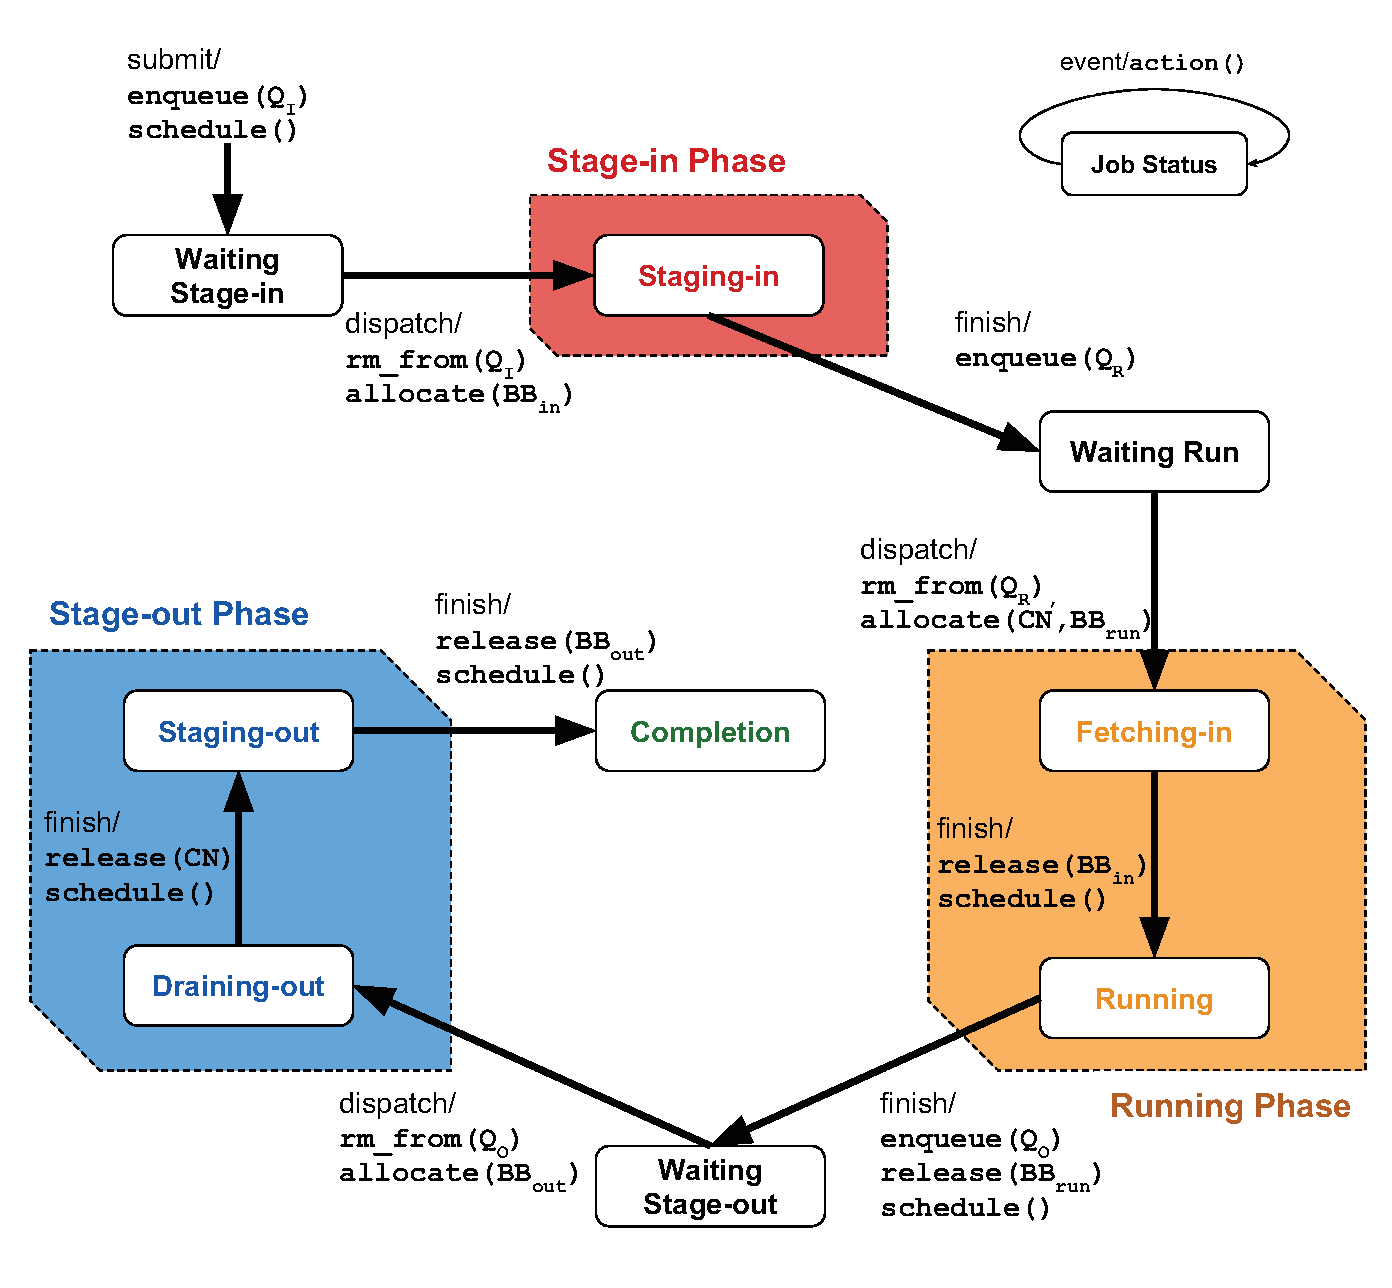
\includegraphics[width=3.6in]{3PhaseJobFSM}
        \caption{Job state transition in Cerberus}
\label{Fig:JobFSM}
\end{figure}

\subsection{Three-Phase Job Scheduling}

The traditional batch scheduler on a system without burst buffer only considers
the job with the number of required nodes and the expected runtime
for making the scheduling decisions.
The most commonly used scheduling policy is the First Come First Serve with EASY backfilling~\cite{tsafrir-tpds-2007}.
However, on burst-buffer-enabled systems,
the amount of available burst buffer capacity becomes a new scheduling constraint.

In this work,
we propose Cerberus, a burst-buffer-aware batch scheduler.
We assume that upon job submission, a user specifies the amount of compute nodes, 
the expected job runtime, and the amount of burst buffer needed by her job.
Cerberus makes scheduling decisions based on the job demands of computing nodes as well as burst buffer.
It allocates burst buffer to each job with regard to its use cases
by maintaining three distinct queues, as shown in Figure~\ref{Fig:CerberusQueues}.
The input queue $Q_I$ contains all the jobs that need to prefetch data
from the external storage to the burst buffer.
The running queue $Q_R$ holds the jobs that are waiting for the compute nodes and
the burst buffer used in data exchange for various purposes.
Jobs waiting to be drained out to the external permanent storage are in the output queue $Q_O$.
The layered hierarchy in Figure~\ref{Fig:CerberusQueues} also indicates that burst buffer
can fill in the memory gap between the memory on compute nodes and the hard disk storage.
Cerberus coordinates three queues and makes scheduling decisions according to job requirements
in each queue with the objective to maximize job performance and system utilization.

%\NOTE{This paragraph moved to start of Section 3}The traditional batch scheduler on a system without burst buffer only considers
%the job with the number of required nodes and the expected runtime for the scheduling decision making process.
%The most commonly used scheduling policy is the First Come First Serve with EASY backfilling~\cite{tsafrir-tpds-2007}.
%However, on burst-buffer-enabled systems,
%the amount of available burst buffer capacity becomes a new scheduling constraint.
%We propose Cerberus, a burst-buffer-aware batch scheduler.
%Cerberus takes the advantage of the most common use cases of burst buffer:
%data stage-in, checkpointing, and data drain-out.
%Cerberus allocates burst buffer in each phase for one of the three use cases
%by maintaining three distinct queues, as shown in Figure~\ref{Fig:CerberusQueues}.
%%Before entering each phase, job must enqueue to the corresponding queue.
%The input queue $Q_I$ contains all the jobs that need to pre-fetch data from the external storage to the burst buffer.
%The running queue $Q_R$ holds the jobs that are waiting for the compute nodes and the burst buffer used for checkpointing.
%Jobs waiting to be drained out to the external permanent storage are in the output queue $Q_O$.
%The layered hierarchy in Figure~\ref{Fig:CerberusQueues} also indicates that burst buffer
%can fill in the memory gap between the memory on compute nodes and the hard disk storage.

To see how Cerberus schedules a particular job by manipulating three queues,
we present the job transition diagram in Figure~\ref{Fig:JobFSM}.
After the submission, a job enters $Q_I$ waiting for the stage-in-purpose burst buffer ($BB_{in}$).
Once selected by Cerberus, the job is removed from $Q_I$ and start to stage input data.
After finishing the stage-in phase, the job is enqueued to $Q_R$,
where it waits for the required compute nodes and \textit{new} burst buffer used in running phase($BB_{run}$).
Note that $BB_{in}$ is still held by the job at this time point.
When Cerberus chooses the job from $Q_R$, the job will be put to the running phase.

The first thing to do in running phase is to release $BB_{in}$ after
\textbf{fetching in} data to the memory of the acquired compute nodes.
During the execution, data exchanges between the memory and the burst buffer $BB_{run}$
may occur frequently.
Once the job execution finishes, $BB_{run}$ can be immediately released since
output data are still available on the compute nodes.
Without releasing the compute nodes, the job enters $Q_O$ and waits for a certain amount of burst buffer for staging out its data ($BB_{out}$).

Once a job in $Q_O$ is chosen by Cerberus, its data flow from the main memory to the burst buffer
in the \textbf{drain-out} sub-phase, after which all the compute nodes can be released.
Then the burst buffer nodes are responsible for transferring the output data to the external storage.
The job completes when all its data are staged out and $BB_{out}$ are returned to system.

As indicated by Figure~\ref{Fig:JobFSM}, the resource release at anytime can trigger Cerberus
to schedule jobs in three queues.
The details of how Cerberus makes scheduling decision for each queue are
described in Section~\ref{SubSec:OptStageIn}-\ref{SubSec:OptStageOut}.
%The fine scheduling granularity enables the full utilization of burst buffer for different purposes.
%The divide-conquer approach provides a framework that can be extended to various scheduling
%policies for each individual phase.
%We propose and solve two optimizations targeting $Q_I/Q_O$ and $Q_R$ in Section~\ref{Sec:Opt}

\subsection{Three-Phase Coordination}
\label{SubSet:Coordination}
The three phase model does not assume data independence between the three phases.
Cooperations are necessary in scheduling the three phases.
First, only after finishing the stage-in phase can a job be ready for running.
Similarly, only when finishing the running phase can a job waiting or entering the stage-out phase,
reflected in the lifetime of a job's execution.
This is still true even when input data is so large that it must be read in in chunks.
In this case we load the first chunk of data in the stage-in phase so that application
can run with one chunk of data;
meanwhile, the application has to keep reading data in chunks during the running phase.
Notice that for this purpose, we only need burst buffer that is able to hold one chunk
of, instead of whole, the input data.
However, this case barely happens because of burst buffer's reasonable capacity\footnote{For
example, 3.7 PB burst buffer on Trinity system should be able to hold most single job's input.}.

Secondly, the burst buffer of any job used at any phase can only be used for a single phase.
For example, a running-phase job cannot hold its already taken burst buffer
and to enter stage-out phase upon finishing the running phase,
regardless whether the holding burst buffer has sufficient capacity.
In Cerberus, the resource release is mandatory as specified in Figure~\ref{Fig:JobFSM}.
We believe that frequent releases provide more opportunities to involve the scheduler in each phase for scheduling the jobs.

Most of the time, data exchanges only between main memory and burst buffer in running phase.
This rule breaks when application generates output data more than main memory's capacity.
When this case occurs, we suggest system put output data chunk first from memory to burst buffer
so that application can resume execution with freed memory;
then we let burst buffer node handle the data transfer to external storage.
Only the last piece of output data are handled in the stage-out phase.

Finally, it is possible that none of three queues are empty at the moment of a scheduling instance.
We choose a heuristic strategy to determine the scheduling order when
Cerberus has to handle multiple queues at the same time.
Note that jobs finishing the \textit{running} and the \textit{stage-out} phases
will (partially) release the resources, and we set the priority of queues to be $priority(Q_O) > priority(Q_R) > priority(Q_I)$.
This greedy heuristic works well when the demand of the jobs in $J_{Q_I}$ is low.
However, it is possible to make jobs stack up at the entry of the system,
whose solution is part of our future work.


\subsection{Scheduling in the Stage-in Phase}
\label{SubSec:OptStageIn}

In the stage-in phase, jobs require only the burst buffer.
Cerberus schedules the jobs in $Q_I$ based on their burst buffer demands $bb\_in$.
To maximize burst buffer's utilization, Cerberus schedules the jobs
according to the following optimization:
\begin{align*}
        \mathbf{Problem} & \text{ } \mathbf{1} \\
        \max &\sum_{i\in J_{Q_I}} bb\_in_i \cdot x_i \\
        s.t. &\left\{
                \begin{array}{l}
                        x_i \in \{0, 1\}, \forall i \in J_{Q_I}\\ [0.8em] \numberthis \label{Equ:MaxTransferData}
                        \sum_{i \in J_{Q_I}} bb\_in_i \cdot x_i \leq BB_{available}
                \end{array}
        \right.
\end{align*}
%\begin{align*}
        %& \max \sum_{i\in S} bb\_in_i \\
        %& s.t. \sum_{i\in S} bb\_in_i \leq BB_{available} \numberthis \label{Equ:MaxTransferData}
        %%\left\{
                %%\begin{array}{l}
                        %%S \subseteq J_{Q_I} \\ [1em]
                        %%\sum_{i\in S} bb\_in_i \leq BB_{available}
                %%\end{array} 
        %%\right.
%\end{align*}
where $J_{Q_I}$ contains all the jobs in the input queue,
$bb\_in_i$ is the burst buffer demand of $job_i$,
$BB_{available}$ is the available capacity of the burst buffer at the moment.
We denote the set of jobs that achieve the maximum data transfer throughput as
$\mathcal{J_{Q_I}} = \{i|x_i = 1, \text{ } \forall i \in J_{Q_I}\}$.

Problem 1 is equivalent to the 0-1 knapsack problem, which is NP-complete.
It can be solved in pseudo-polynomial time through dynamic programming and backtracking.
Memorization technique is applied in order to accelerate the solving process.
The recursive relationship used in our solution is given by \equref{Equ:MaxTransferDataRecursion}.
The time complexity of solving \equref{Equ:MaxTransferDataRecursion} and 
backtracking $\mathcal{J}_{Q_I}$ is $O(n\times BB)$.


\subsection{Scheduling in the Running Phase}
\label{SubSec:OptRunning}
Running jobs not only require the compute nodes for computation,
but also utilize the burst buffer to enhance the I/O performance.
Here we take a general strategy by defining the \textbf{profit} of $job_i$
in $Q_R$ as it uses $c_i$ compute nodes and $bb\_run_i$ amount of the burst buffer
\begin{equation}
        p_i = f(c_i, bb\_run_i, ert_i)
\label{Equ:GeneralProfit}
\end{equation}
where $ert_i$ is the expected running time of $job_i$.

Cerberus's objective is to maximize the total profit of jobs in the running queue, formularized as
\begin{align*}
        \mathbf{Problem} & \text{ } \mathbf{2} \\
        \max &\sum_{i \in J_{Q_R}} p_i \cdot x_i \\
        s.t. &\left\{
                \begin{array}{l}
                        x_i \in \{0, 1\}, \forall i \in J_{Q_R} \\ [0.8em]
                        \sum_{i \in J_{Q_R}} c_i \cdot x_i \leq CN_{available} \\ [0.8em]\numberthis \label{Equ:MaxProduct} 
                        \sum_{i \in J_{Q_R}} bb\_run_i \cdot x_i \leq BB_{available}
                \end{array} 
        \right.
\end{align*}
where $J_{Q_R}$ contains all the jobs in the running queue,
$CN_{available}$ and $BB_{available}$ represent the amount of system's current available resources.
We denote the set of jobs who have the maximum profit as
$\mathcal{J}_{Q_R}  = \{i|x_i=1, \text{ } \forall i \in J_{Q_R}\}$.

As an example, we measure the value of a job based on how efficient one utilizes its resource:
\begin{equation}
        p_i = \frac{c_i / CN}{ert_i} \times \frac{bb\_run_i / BB}{ert_i}
        \label{Equ:DefValue}
\end{equation}
In \equref{Equ:DefValue}, efficiency is measured as the ratio
of the job resource demand to the expected job running time,
where the share of the requested compute nodes ($c_i/CN$) and
the share of the requested burst buffer ($bb\_run/BB$) are used to
represent the demand size.
Specializing Problem 2 using \equref{Equ:DefValue} in fact favors tasks that claim to take up the resources with a short duration, as we will discuss in Section~\ref{Sec:Experiments}.
%\begin{align*}
        %& \max \sum_{i \in S}\frac{c_i}{ert_i} * \frac{bb\_run_i}{ert_i} \\
        %& s.t. \left\{
                %\begin{array}{l}
                        %%S \subseteq J_{Q_R} \\ [1em]
                        %\sum_{i \in S} c_i \leq CN_{available} \\ [0.5em]\numberthis \label{Equ:MaxProduct} 
                        %\sum_{i \in S} bb\_run_i \leq BB_{available}
                %\end{array} 
        %\right.
%\end{align*}


Problem 2 can be informally treat as the two-dimension 0-1 knapsack problem.
We use the same dynamic programming skill to solve Problem 2.
The recursion is given by \equref{Equ:MaxProductRecursion}.
The time complexity of solving \equref{Equ:MaxProductRecursion} and selecting $\mathcal{J}_{Q_R}$ with memorization technique is $O(n\times CN\times BB)$.


\subsection{Scheduling in the Stage-out Phase}
\label{SubSec:OptStageOut}

The stage-out phase scheduling is designed based on the value of $bb\_out$ of the jobs in $Q_O$.
The optimization formula for the stage-out phase is the same as Problem 1, 
except that $bb\_in_i$ is replaced with $bb\_out_i$, 
and $J_{Q_I}$ is replaced with $J_{Q_O}$, the job set of output queue.
The solution is also extremely similar to \equref{Equ:MaxTransferDataRecursion} and
has the same $O(n\times BB)$ time complexity.


%\subsection{Solving the Optimization Problems}
%
%Problem 2 can be informally treat as the 2-dimension 0-1 knapsack problem.
%We expect all of them to be NP-hard problems.
%Dynamic programming is adopted to solve them in pseudo-polynomial time.
%Applying memorization could also help accelerate the solving process.
%In addition, we are not interested in the optimal result of
%Problem 1 and Problem 2,
%but in a combination of jobs $\mathcal{J}$ that yields to the optimal solution,
%which, fortunately, can also be tracked back down using the memorizations stored during the dynamic programming execution.
%
%For Problem 1, the recursive relationship is given by \equref{Equ:MaxTransferDataRecursion}.
%The recursion that solves Problem 2 is given by \equref{Equ:MaxProductRecursion}.
%Solving \equref{Equ:MaxTransferDataRecursion} and 
%backtracking $\mathcal{J}_{Q_I}$ or $\mathcal{J}_{Q_O}$ in total take time proportional to $n\times BB$.
%Similarly, solving \equref{Equ:MaxProductRecursion} and selecting $\mathcal{J}_{Q_R}$ using memo
%are $O(n\times CN\times BB)$.


\begin{strip}
        \begin{align}
                dp(i, w) = & 
                \left\{
                        \begin{array}{l}
                                0, \text{ if $i=0$ } \\ [0.6em]
                                dp(i-1, w), \text{ if $bb\_in_i > w$} \\ [0.6em]
                                \max \{ dp(i-1, w), dp(i-1, w-bb\_in_i) + bb\_in_i \}, \text{ if $bb\_in_i \leq w$}
                        \end{array} 
                \right.
                \label{Equ:MaxTransferDataRecursion} 
        \end{align}
\end{strip}

\begin{strip}
        \begin{align}
                dp(i, c, w) = &
                \left\{
                        \begin{array}{l}
                                0, \text{ if $i=0$ } \\ [0.6em]
                                dp(i-1, c, w), \text{ if $c_i > c$ or $bb\_run_i > w$} \\ [0.6em]
                                \max \{ dp(i-1, c, w), dp(i-1, c - c_i, w - bb\_run_i) + p_i \}, \text{ if $c_i \leq c$ and $bb\_run_i \leq w$}
                        \end{array} 
                \right.
                \label{Equ:MaxProductRecursion}
        \end{align}
\end{strip}

\subsection{Discussion}
The optimal solutions in any of scheduling phases may not be unique;
then backtracking via memoization only yields one of the optimal solution to Problem 1-3.
For example, backtracking $\mathcal{J}_{Q_R}$ using $dp(i,c,w)$ can only return 1 scheduling
configuration that maximize our optimization goal.
If the runtime system designer don't specify extra constraints in the scheduling problems,
Cerberus, as any other scheduler, cannot automatically prioritize \textbf{optimal} solutions
because prioritizing using any hidden rules leads to some kind of unfairness.

Another thing to point out is that Cerberus is \textbf{NOT} unfair to non-I/O jobs.
As for Problem 1, a non-I/O job will always be selected by Cerberus.
Since we have $bb_{in} = 0$ for non-I/O jobs, adding it to $\mathcal{J}_{Q_I}$ will affect
neither of the constraints in \equref{Equ:MaxTransferData}.
To avoid starving certain jobs demanding extremely large number of burst buffers and/or cores,
Cerberus keeps tracking of their holding time.
When the waiting time exceed certain threshold, Cerberus will stop the normal scheduling
process to ensure dispatching the large jobs.





%% \subsection{Optimize Stage-in Phase}
% In the stage-in phase, only burst buffer demand is considered.
% Scheduling is made based on the value of $bb\_in$ of jobs in $Q_I$.
% If we care about data transfer throughput,
% we should transfer as much data as possible by doing the following optimization:
% \begin{align*}
%         & \max \sum_{i\in S} bb\_in_i \\
%         & s.t. \sum_{i\in S} bb\_in_i \leq BB_{available} \numberthis \label{Equ:MaxTransferData}
%         %\left\{
%                 %\begin{array}{l}
%                         %S \subseteq J_{Q_I} \\ [1em]
%                         %\sum_{i\in S} bb\_in_i \leq BB_{available}
%                 %\end{array} 
%         %\right.
% \end{align*}
% where $J_{Q_I}$ stands for all jobs in input queue at the time considering,
% $S\subseteq J_{Q_I}$ is the set of job selected by Cerberus,
% $bb\_in_i$ is the burst buffer demand of $job_i$,
% $BB_{available}$ is system's available amount of burst buffer.
% 
% Stage-out phase scheduling are made based on the value of $bb\_out$ of jobs in $Q_O$.
% Optimization formula for different purpose are almost the same as
% Equation~\ref{Equ:MaxTransferData},
% except that $bb\_in$ is replaced with $bb\_out$,
% $J_{Q_I}$ is replaced with $J_{Q_O}$, the job set of output queue.


\section{Optimization Enhancement}
\label{Sec:Opt}

Cerberus can be further enhanced using various optimizations
when making the scheduling decisions for jobs in each queue.
This section defines two types of optimization techniques used for scheduling jobs in one of the three phases.
We compute the solutions using dynamic programming.

\subsection{Scheduling Optimization in Stage-in Phase}

In the stage-in phase, jobs require only the burst buffer.
Cerberus schedules the jobs in $Q_I$ based on their burst buffer demands $bb\_in$.
To maximize burst buffer's utilization, one can schedule the jobs according to the following optimization:
\begin{align*}
        \mathbf{Problem} & \text{ } \mathbf{1} \\
        \max &\sum_{i\in J_{Q_I}} bb\_in_i \cdot x_i \\
        s.t. &\left\{
                \begin{array}{l}
                        x_i \in \{0, 1\}, \forall i \in J_{Q_I}\\ [0.8em] \numberthis \label{Equ:MaxTransferData}
                        \sum_{i \in J_{Q_I}} bb\_in_i \cdot x_i \leq BB_{available}
                \end{array}
        \right.
\end{align*}
%\begin{align*}
        %& \max \sum_{i\in S} bb\_in_i \\
        %& s.t. \sum_{i\in S} bb\_in_i \leq BB_{available} \numberthis \label{Equ:MaxTransferData}
        %%\left\{
                %%\begin{array}{l}
                        %%S \subseteq J_{Q_I} \\ [1em]
                        %%\sum_{i\in S} bb\_in_i \leq BB_{available}
                %%\end{array} 
        %%\right.
%\end{align*}
where $J_{Q_I}$ stands for all jobs in the input queue,
$bb\_in_i$ is the burst buffer demand of $job_i$,
$BB_{available}$ is the system's current available capacity of the burst buffer.
We denote the set of jobs that achieve the maximum data transfer throughput as
$\mathcal{J} = \{x_i|x_i = 1, \text{ } \forall i \in J_{Q_I}\}$.


% \subsection{Optimize Running Phase}
% Running jobs require not only compute nodes, but burst buffer to ensure performance and correctness.
% Scheduling are accordingly made based on the value of $c$ and $bb\_run$ of jobs in $Q_R$.
% To maximize multiple types of resource's utilization,
% we convert it to the knapsack problem by defining the value of the $job_i$ as
% \begin{equation}
%         v_i = \frac{c_i / CN}{rt_i} \times \frac{bb\_run_i / BB}{rt_i}
%         \label{Equ:DefValue}
% \end{equation}
% where $rt_i$ is the running time of $job_i$, the time it takes up the computing nodes.
% By defining \textit{value} as Equation~\ref{Equ:DefValue},
% we prefer these tasks that claims to take up node resources with short duration.
% Unfortunately, it is difficult to predict $rt_i$ before actually running the job.
% Of course we could use the \textit{expected running time} $ert_i$ specified by user.
% However, by examining the log traces from Argonne National Laboratory (ANL)\cite{JobTrace},
% we found that the variance between $rt_i$ and $ert_i$ is significantly different.
% For now we can just assume $ert_i$ represent $rt_i$ of $job_i$.
% In the future, we could adopt machine learning or data mining ideas
% to predict the running time of a job with demand vector.
% %Notice that then the value of a task is proportional to $c_i*bb_i$.
% The optimizing formula can thus be
% \begin{align*}
%         & \max \sum_{i \in S}\frac{c_i}{ert_i} * \frac{bb\_run_i}{ert_i} \\
%         & s.t. \left\{
%                 \begin{array}{l}
%                         %S \subseteq J_{Q_R} \\ [1em]
%                         \sum_{i \in S} c_i \leq CN_{available} \\ [0.5em]\numberthis \label{Equ:MaxProduct} 
%                         \sum_{i \in S} bb\_run_i \leq BB_{available}
%                 \end{array} 
%         \right.
% \end{align*}
% where $J_{Q_R}$ is the set of jobs in running queue,
% $S\subseteq J_{Q_R}$ stands for jobs selected by scheduler,
% $CN_{available}$ and $BB_{available}$ represent the amount of system's available resources
% (compute nodes and burst buffer nodes) at current moment.



\subsection{Scheduling Optimization in Running Phase}
Running jobs not only require the compute nodes for computation,
but also utilize the burst buffer to enhance the I/O performance.
Here we take a general strategy by defining the \textbf{profit} of $job_i$
in $Q_R$ as it uses $c_i$ compute nodes and $bb\_run_i$ amount of the burst buffer
\begin{equation}
        p_i = f(c_i, bb\_run_i, ert_i)
\label{Equ:GeneralProfit}
\end{equation}
where $ert_i$ is the expected running time of $job_i$.

Similar to the 0-1 knapsack problem, the objective is to maximize the total profit of jobs in the running queue, formularized as
\begin{align*}
        \mathbf{Problem} & \text{ } \mathbf{2} \\
        \max &\sum_{i \in J_{Q_R}} p_i \cdot x_i \\
        s.t. &\left\{
                \begin{array}{l}
                        x_i \in \{0, 1\}, \forall i \in J_{Q_R} \\ [0.8em]
                        \sum_{i \in J_{Q_R}} c_i \cdot x_i \leq CN_{available} \\ [0.8em]\numberthis \label{Equ:MaxProduct} 
                        \sum_{i \in J_{Q_R}} bb\_run_i \cdot x_i \leq BB_{available}
                \end{array} 
        \right.
\end{align*}
where $J_{Q_R}$ is the set of jobs in the running queue,
$CN_{available}$ and $BB_{available}$ represent the amount of system's current available resources.
We denote the set of jobs who have the maximum profit as
$\mathcal{J}  = \{x_i|x_i=1, \text{ } \forall i \in J_{Q_R}\}$.

As an example, we measure the value of a job based on how efficient one utilize its resource:
\begin{equation}
        p_i = \frac{c_i / CN}{ert_i} \times \frac{bb\_run_i / BB}{ert_i}
        \label{Equ:DefValue}
\end{equation}
Here, efficiency is measured as the ratio of the job resource demand to the expected job running time,
where the share of the requested compute nodes ($c_i/CN$) and the burst buffer ($bb\_run/BB$) are used to
represent the demand size.
Specializing Problem 2 using \equref{Equ:DefValue} in fact favors tasks that claim to take up the resources with a short duration, as we will discuss in Section~\ref{Sec:Experiments}.
%\begin{align*}
        %& \max \sum_{i \in S}\frac{c_i}{ert_i} * \frac{bb\_run_i}{ert_i} \\
        %& s.t. \left\{
                %\begin{array}{l}
                        %%S \subseteq J_{Q_R} \\ [1em]
                        %\sum_{i \in S} c_i \leq CN_{available} \\ [0.5em]\numberthis \label{Equ:MaxProduct} 
                        %\sum_{i \in S} bb\_run_i \leq BB_{available}
                %\end{array} 
        %\right.
%\end{align*}

\subsection{Scheduling Optimization in Stage-out Phase}

The stage-out phase scheduling is designed based on the value of $bb\_out$ of the jobs in $Q_O$.
The optimization formula for the stage-out phase are almost the same as the ones in Problem 1, except that $bb\_in_i$ is replaced with $bb\_out_i$, and
$J_{Q_I}$ is replaced with $J_{Q_O}$, the job set of output queue.


\subsection{Solving the Optimization Problems}
% It is trivial to show that optimization problem~\ref{Equ:MaxTransferData}
% is equivalent to 0-1 knapsack problem.
% Problem~\ref{Equ:MaxProduct} can be informally treat as 2-dimension 0-1 knapsack problem.
% We expect all of them are NP-hard problems.
% We can solve them with dynamic programming in pseudo polynomial time.
% Applying memorization could also help accelerate the solving process.
% However, we are not interested in the optimal result of
% problem~\ref{Equ:MaxTransferData} and problem~\ref{Equ:MaxProduct}
% but in a combination of jobs that yields the optimal solution,
% which, fortunately, can also be tracked back down
% using the memorizations kept in dynamic programming.

% %The solution to Problem~\ref{Equ:MaxTransferData},
% %Problem~\ref{Equ:MaxTaskNumber} and Problem~\ref{Equ:MaxProduct} are similar.
% First, for Problem~\ref{Equ:MaxTransferData}, the recursive relationship is
% given by Recursion~\ref{Equ:MaxTransferDataRecursion}.
% In~\ref{Equ:MaxTransferDataRecursion}, the memo we keeps during solving is
% the optimal solution for 
% $jobs=(job_1, job_2, \ldots, job_i)$ with $w$ GB of available burst buffer.
% For Problem~\ref{Equ:MaxProduct}, we keep the memo of the optimal solution 
% for $jobs=(job_1, job_2, \ldots, job_i)$
% with $c$ computing nodes and $w$ GB of burst buffer being available.

% Scheduler can obtain an optimal combination of jobs by tracking along the memo.
% Take the problem~\ref{Equ:MaxProduct} problem for example.
% We start from $dp(n, CN, BB)$.
% If $c_n \leq CN$ and $bb\_in_n \leq BB$, $job_n$ should be scheduled if
% $dp(i-1, c, w) \leq dp(i-1, c - c_i, w - bb\_in_i) + c_i bb\_in_i$ and
% recurse with $dp(n - 1, CN - c_i, BB - bb\_in_i)$;
% otherwise, $job_n$ should be skipped and we recurse the process on $dp(n-1, CN, BB)$.
% The time complexity of solving Recursion~\ref{Equ:MaxTransferDataRecursion} is $O(n\times BB)$.
% The time complexity of solving Recursion~\ref{Equ:MaxProductRecursion}
% is $O(n\times CN\times BB)$.

% Notice that $CN$ and $BB$ may be very large integers,
% making the pseudo-polynomial algorithm unsuitable
% to be used online by scheduler.
% In practice, we could reduce the time complexity by allocating resource
% in a coarser granularity.
% For example, jobs usually asks for compute node in the unit of $cn\_unit = 512$ nodes;
% demands for burst buffer nodes on checkpointing and output are
% usually in the unit of $bb\_unit = 1$ TB.
% We can divide both $CN$ and $c_i$ by $cn\_unit$;
% divide both $BB$ and $bb\_run, bb\_out$ by $bb\_unit$.
% It is also possible to reduce the value of $n$, the number of jobs in the queue.
% For example, we can consider only $\frac{1}{\alpha}n$ jobs in the queue.
% This will give us only the partial optimal solution
% in exchange of less computation complexity.

It is trivial to show that the optimization of Problem 1
is equivalent to the 0-1 knapsack problem.
Problem 2 can be informally treat as the 2-dimension 0-1 knapsack problem.
We expect all of them to be NP-hard problems.
Dynamic programming is adopted to solve them in pseudo-polynomial time.
Applying memorization could also help accelerate the solving process.
In addition, we are not interested in the optimal result of
Problem 1 and Problem 2,
but in a combination of jobs $\mathcal{J}$ that yields to the optimal solution,
which, fortunately, can also be tracked back down using the memorizations stored during the dynamic programming execution.
%How to fill in memo and track back optimal $\mathcal{J}$ are shown in Algorithm~\ref{Alg:MaxBB}
%and Algorithm~\ref{Alg:MaxCPU} for Problem 1
%and Problem 2 respectively.
%The time complexity of Algorithm~\ref{Alg:MaxBB} is $O(n\times BB)$.
%The time complexity of solving Algorithm~\ref{Alg:MaxCPU} is $O(n\times CN\times BB)$.
For Problem 1, the recursive relationship is given by \equref{Equ:MaxTransferDataRecursion}.
The recursion that solves Problem 2 is given by \equref{Equ:MaxProductRecursion}.
Solving \equref{Equ:MaxTransferDataRecursion} and 
backtracking $\mathcal{J}_{Q_I}$ or $\mathcal{J}_{Q_O}$ in total take time proportional to $n\times BB$.
Similarly, solving \equref{Equ:MaxProductRecursion} and selecting $\mathcal{J}_{Q_R}$ using memo
are $O(n\times CN\times BB)$.


\begin{strip}
        \begin{align}
                dp(i, w) = & 
                \left\{
                        \begin{array}{l}
                                0, \text{ if $i=0$ } \\ [0.6em]
                                dp(i-1, w), \text{ if $bb\_in_i > w$} \\ [0.6em]
                                \max \{ dp(i-1, w), dp(i-1, w-bb\_in_i) + bb\_in_i \}, \text{ if $bb\_in_i \leq w$}
                        \end{array} 
                \right.
                \label{Equ:MaxTransferDataRecursion} 
        \end{align}
\end{strip}

\begin{strip}
        \begin{align}
                dp(i, c, w) = &
                \left\{
                        \begin{array}{l}
                                0, \text{ if $i=0$ } \\ [0.6em]
                                dp(i-1, c, w), \text{ if $c_i > c$ or $bb\_run_i > w$} \\ [0.6em]
                                \max \{ dp(i-1, c, w), dp(i-1, c - c_i, w - bb\_run_i) + p_i \}, \text{ if $c_i \leq c$ and $bb\_run_i \leq w$}
                        \end{array} 
                \right.
                \label{Equ:MaxProductRecursion}
        \end{align}
\end{strip}


%\algrenewcommand{\algorithmiccomment}[1]{\hskip1em$/*$ #1 $*/$}

%\begin{algorithm}[t]
%\caption{Maximize Data Transfer of Jobs in $Q_I$ or $Q_O$}
%\label{Alg:MaxBB}
%\begin{algorithmic}[1]
        %\State $\boldsymbol{bb} \gets $ burst buffer demands of $J_Q$
        %\State $\boldsymbol{dp} \gets \boldsymbol{0}_{(N+1) \times (BB+1)}$
        %\State $\mathcal{J} \gets \emptyset$\Comment{scheduling result}
        %\\
        %\Function{FillInMemo}{ }
                %\For{$i \gets 1, N$}
                        %\For{$w \gets 1, BB$}
                                %\If{$w \geq bb_i$}
                                        %\State $dp_1 = dp(i-1, w-bb_i)+bb_i$
                                        %\State $dp_2 = dp(i-1, w)$
                                        %\State $dp(i, w) \gets \max\{dp_1, dp_2\}$
                                %\Else
                                        %\State $dp(i,w) \gets dp(i-1,w)$
                                %\EndIf
                        %\EndFor
                %\EndFor
                %\State \Call{TrackBackJobs}{$N, BB$}
        %\EndFunction
        %\\
        %\Function{TrackBackJobs}{$i, w$}
                %\If{$i > 0$}
                        %\If{$w \geq bb_i$}
                                %\State $dp_1 = dp(i-1, w-bb_i)+bb_i$
                                %\State $dp_2 = dp(i-1, w)$
                                %\If{$dp_1 \geq dp_2$}
                                        %\State $\mathcal{J} = \mathcal{J} \cup job_i$
                                        %\State \Call{TrackBackJobs}{$i-1, w-bb_i$}
                                %\Else
                                        %\State \Call{TrackBackJobs}{$i-1, w$}
                                %\EndIf
                        %\Else
                                %\State \Call{TrackBackJobs}{$i-1, w$}
                        %\EndIf
                %\EndIf
        %\EndFunction
%\end{algorithmic}
%\end{algorithm}

%\begin{algorithm}[t]
%\caption{Maximize Profit of Jobs in $Q_R$}
%\label{Alg:MaxCPU}
%\begin{algorithmic}[1]
        %\State $\boldsymbol{bb} \gets $ burst buffer demands of $J_Q$
        %\State $\boldsymbol{cn} \gets $ compute nodes demands of $j \in J_Q$
        %\State $\boldsymbol{dp} \gets \boldsymbol{0}_{(N+1) \times (CN) \times (BB+1)}$
        %\State $\boldsymbol{v} \gets$ values of $j \in J_Q$
        %\State $\mathcal{J} \gets \emptyset$\Comment{scheduling result} 
        %\\
        %\Function{FillInMemo}{ }
                %\For{$i \gets 1, N$}
                        %\For{$c \gets 1, CN$} 
                                %\For{$w \gets 1, BB$}
                                        %\If{$c \geq cpu_i$ and $w \geq bb_i$}
                                                %\State $dp_1 = dp(i-1, c-cn_i, w-bb_i)+v_i$
                                                %\State $dp_2 = dp(i-1, c, w)$
                                                %\State $dp(i, c, w) \gets \max\{dp_1, dp_2\}$
                                        %\Else
                                                %\State $dp(i,c,w) \gets dp(i-1,c,w)$
                                        %\EndIf
                                %\EndFor
                        %\EndFor
                %\EndFor
                %\State \Call{TrackBackJobs}{$N, CN, BB$}
        %\EndFunction
        %\\
        %\Function{TrackBackJobs}{$i, c, w$}
                %\If{$i > 0$}
                        %\If{$c \geq cpu_i$ and $w \geq bb_i$}
                                %\State $dp_1 = dp(i-1, c-cn_i, w-bb_i)+v_i$
                                %\State $dp_2 = dp(i-1, c, w)$
                                %\If{$dp_1 \geq dp_2$}
                                        %\State $\mathcal{J} = \mathcal{J} \cup job_i$
                                        %\State \Call{TrackBackJobs}{$i-1, c-cpu_i, w-bb_i$}
                                %\Else
                                        %\State \Call{TrackBackJobs}{$i-1, c, w$}
                                %\EndIf
                        %\Else
                                %\State \Call{TrackBackJobs}{$i-1, c, w$}
                        %\EndIf
                %\EndIf
        %\EndFunction
%\end{algorithmic}
%\end{algorithm}




% \section{Event-driven Burst Buffer Simulator}
% \label{Sec:Simulation}

% We develop an event-driven simulator for burst buffer enabled HPC system, named \textbf{BBSim},
% from scratch in Python to mimic Cerberus scheduling Trinity.\NOTE{Fig has no info about Trinity}
% It roughly consists of 1,400 lines of code.
% Figure~\ref{Fig:JobFSM} illustrates the simulation lifetime of a job in BBSim
% using extended finite state machine (EFSM).
% The \textit{state} of the job changes depending on current status and
% happening \textit{events}, along with which an \textit{action} is taken.
% For example, at the very beginning, submitted $job_i$ will enter \textbf{Waiting Stage-in} state;
% at the meanwhile, $job_i$ is enqueued to $Q_I$ and scheduler is triggered to do scheduling.

\section{BBSim: An Event Driven Simulator of Cerberus}
\label{Sec:Simulation}

We develop an event-driven simulator, named \textbf{BBSim},
to simulate how Cerberus schedules jobs on burst-buffer-enabled HPC systems.
Apart from demonstrating the lifetime of a job scheduled by Cerberus,
Figure~\ref{Fig:JobFSM} also illustrates the various events in BBSim and how to handle
them in an event-driven-simulation approach.
The transitions of job \textit{state}, along with which an \textit{action} is triggered,
depend on the current state and the \textit{event} happened.
For example, when $job_i$ is submitted to the system,
it enters the \textit{Waiting Stage-in} state,
waiting to be scheduled in the job queue $Q_I$. 
The scheduler checks $job_i$'s resource demand and
dispatches it to run when sufficient resources are available.

% Whenever job enters one of its 3 phases, system resources are allocated:
% \begin{itemize}
%         \item $BB_{in}$ TB amount of burst buffer are allocated upon entering stage-in phase.
%         \item $CN$ number of compute nodes and $BB_{run}$ amount of burst buffer
%                 are allocated upon entering running phase.
%         \item $BB_{out}$ TB of burst buffer are allocated upon entering stage-out phase.
% \end{itemize}
% Various \texttt{release()} actions are of importance because, in addition to submission,
% \texttt{schedule()} is invoked to schedule waiting jobs
% whenever system resources are released:
% \begin{itemize}
%         \item When job's data is loaded from burst buffer to memory,
%                 burst buffer allocated at stage-in phase are released.
%         \item When job finishes running, system reclaims burst buffer nodes
%                 used for checkpointing.
%         \item When job's data is written to burst buffer from memory,
%                 compute nodes taken by job are returned.
%         \item When job's data is staged out to external disk,
%                 its burst buffer nodes are released.
% \end{itemize}
% 
% \begin{figure}[!t]
% \centering
%         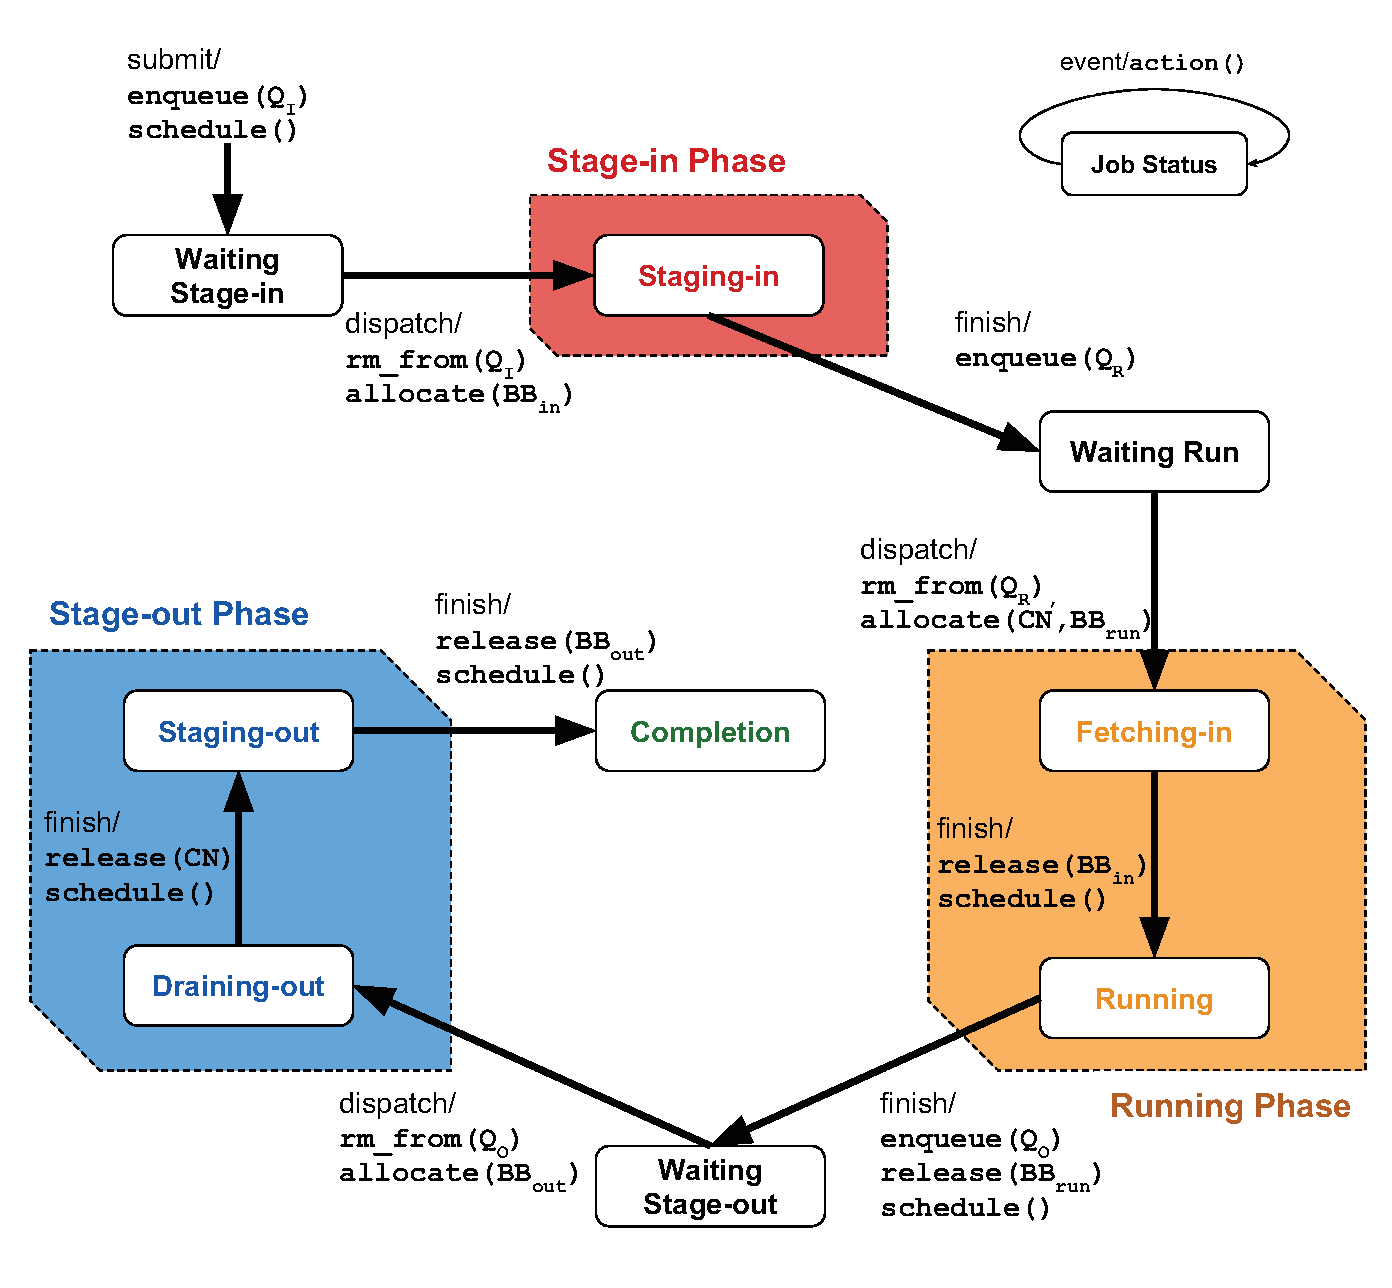
\includegraphics[width=3.6in]{3PhaseJobFSM}
%         \caption{Finite State Machine of Scheduling Simulation}
% \label{Fig:JobFSM}
% \end{figure}


%Whenever $job_i$ enters one of the three phases, the system resources are allocated in the following way:
%\begin{itemize}
        %\item $BB_{in}$ TB amount of burst buffer are allocated upon entering the stage-in phase.
        %\item $CN$ number of compute nodes and $BB_{run}$ amount of burst buffer
                %are allocated upon entering the running phase.
        %\item $BB_{out}$ TB of burst buffer is allocated upon entering the stage-out phase.
%\end{itemize}

Various \texttt{release()} actions are important because, in addition to job submissions,
\texttt{schedule()} will be invoked to schedule the waiting jobs.
The allocated resource can only be released when one phase is finished.
Therefore, any \textit{dispatch} event, generated by the \texttt{schedule()} action,
follows a certain \textit{finish} event.
The allocated resources are released at the following time points:
\begin{itemize}
        \item When $job_i$ pre-fetches data from the burst buffer to the memory,
                the burst buffer allocated in the stage-in phase ($BB_{in}$) is released.
        \item When $job_i$ completes the computation,
                the system reclaims the burst buffer allocated in the running phase ($BB_{run}$).
        \item When $job_i$ output data is written to the burst buffer from the memory,
              compute nodes ($CN$) allocated in the running phase are released.
        \item When output data are drained out to the external storage,
                the burst buffer allocated in the stage-out phase ($BB_{out}$) is released.
                The simulation for $job_i$ completes.
\end{itemize}




% Notice that resource can only be released when certain phase is finished.
% Therefore, any \textit{dispatch} event, caused by \texttt{schedule()} action, actually happens
% at the meanwhile of a certain \textit{finish} event.
% The timestamps of all possible \textit{finish} events are calculated in the following way:
% \begin{align}
%         & TS_{f\_stagein} = TS_{s\_stagein} + \frac{bb\_in}{BW_{io\_to\_bb}}\label{Equ:FinIn} \\
%         & TS_{f\_loadin} = TS_{s\_run} + \frac{bb\_in}{BW_{bb\_to\_cn}}\label{Equ:FinMemIn} \\
%         & TS_{f\_run} = TS_{f\_loadin} + \frac{bb\_run}{BW_{cn\_to\_bb}} + rt\label{Equ:FinRun} \\
%         & TS_{f\_loadout} = TS_{s\_stageout} + \frac{bb\_out}{BW_{cn\_to\_bb}}\label{Equ:FinMemOut} \\
%         & TS_{f\_stageout} = TS_{f\_loadout} + \frac{bb\_out}{BW_{bb\_to\_io}} \label{Equ:FinOut}
% \end{align}
% where $TS_{f\_x}$ stands for the timestamps of finishing phase $x$,
% $TS_{s\_x}$ stands for the timestamps of starting phase $x$,
% $BW_{x\_to\_y}$ stands for the bandwidth between $x$ and $y$.
% 
% Though target on burst buffer system, BBSim also supports simulating non-BB HPC system.
% Besides, it is not coupled with Cerberus but easy to simulating many other scheduler.
% Both can be proved by the following experiments for various schedulers.


%The timestamps of all the \textit{finish} events are calculated as follows:
%\begin{align}
%        & TS_{f\_stagein} = TS_{s\_stagein} + \frac{bb\_in}{BW_{io\_to\_bb}}\label{Equ:FinIn} \\
%        & TS_{f\_loadin} = TS_{s\_run} + \frac{bb\_in}{BW_{bb\_to\_cn}}\label{Equ:FinMemIn} \\
%        & TS_{f\_run} = TS_{f\_loadin} + \frac{bb\_run}{BW_{cn\_to\_bb}} + rt\label{Equ:FinRun} \\
%        & TS_{f\_loadout} = TS_{s\_stageout} + \frac{bb\_out}{BW_{cn\_to\_bb}}\label{Equ:FinMemOut} \\
%        & TS_{f\_stageout} = TS_{f\_loadout} + \frac{bb\_out}{BW_{bb\_to\_io}} \label{Equ:FinOut}
%\end{align}
%where $TS_{f\_x}$ stands for the timestamps of the finishing phase $x$,
%$TS_{s\_x}$ stands for the timestamps of the starting phase $x$,
%$BW_{x\_to\_y}$ stands for the bandwidth between $x$ and $y$.
%BBSim does not simulate the data transfer between I/O nodes and PFS through the network.

% % system
% We consider simulating the full Trinity super computer\cite{TrinitySystem}.
% The number of compute nodes on Trinity is about 18,936,
% e.g. 9,436 Intel Haswell nodes
% and at least 9500 Intel Xeon Phi nodes.
% There are 16 cores on each processor, thus totally 302,976 cores.
% In the following experiments, we compare two identical system except that
% I/O nodes are replaced by the same number of burst buffer nodes.
% Eventually Trinity plans to delivery up to 576 burst buffer nodes of 3.7 PB,
% consisted of Trinity I/O nodes with PCIe SSD card.
% They are globally accessible as intermediate storage and distributed among cabinets.
% Sequential read/write speed of burst buffer nodes is 8.0 GBps.
% Bandwidth between CPU node and non-burst-buffer I/O node is set to 2.5 GBps.


Our Python implementation of BBSim includes three major modules.
The \texttt{simulator} module drives the event-driven simulation process.
Various job models, job demands, and schedulers are in \texttt{scheduler} module.
The \texttt{dp\_solver} module provides dynamic programming solutions for
the \texttt{Cerberus} scheduler in \texttt{scheduler}.
Though targeting on burst buffer enabled systems,
BBSim also supports simulating job scheduling on HPC systems without burst buffer.
Besides, it is easy to integrate other scheduling policies into BBSim.
The codebase of BBSim and Cerberus are made public to the community\cite{bbsim-github}.


We use BBSim to simulate
a burst-buffer-enabled HPC system shown in Figure~\ref{Fig:BBArchitecture}.
The system adopts traditional IBM Blue Gene/P architecture but burst buffer are
assumably available in the I/O nodes.
We simulate a system consists of 18,936 compute nodes,
e.g., 9,436 Intel Haswell nodes and 9,500 Intel Xeon Phi nodes.
The parameters related to burst buffer are taken from the 
NERSC-8 Use Case Scenarios technical report\cite{BBUseCase} on Trinity system\cite{TrinitySystem},
the next generation supercomputer in Los Alamos National Laboratory.
Specifically, there are 576 burst buffer enabled nodes with aggregated 3.7 PB storage,
which are globally accessible as the intermediate storage.
The sequential read/write speed of burst buffer nodes is 8.0 GBps.
The bandwidth between a CPU node and an I/O node is set to 2.5 GBps.
The time spent for job's I/O operation in our simulation is calculated by
dividing the amount of transferred data by the corresponding bandwidth.

\begin{figure}[htp]
        \centering
        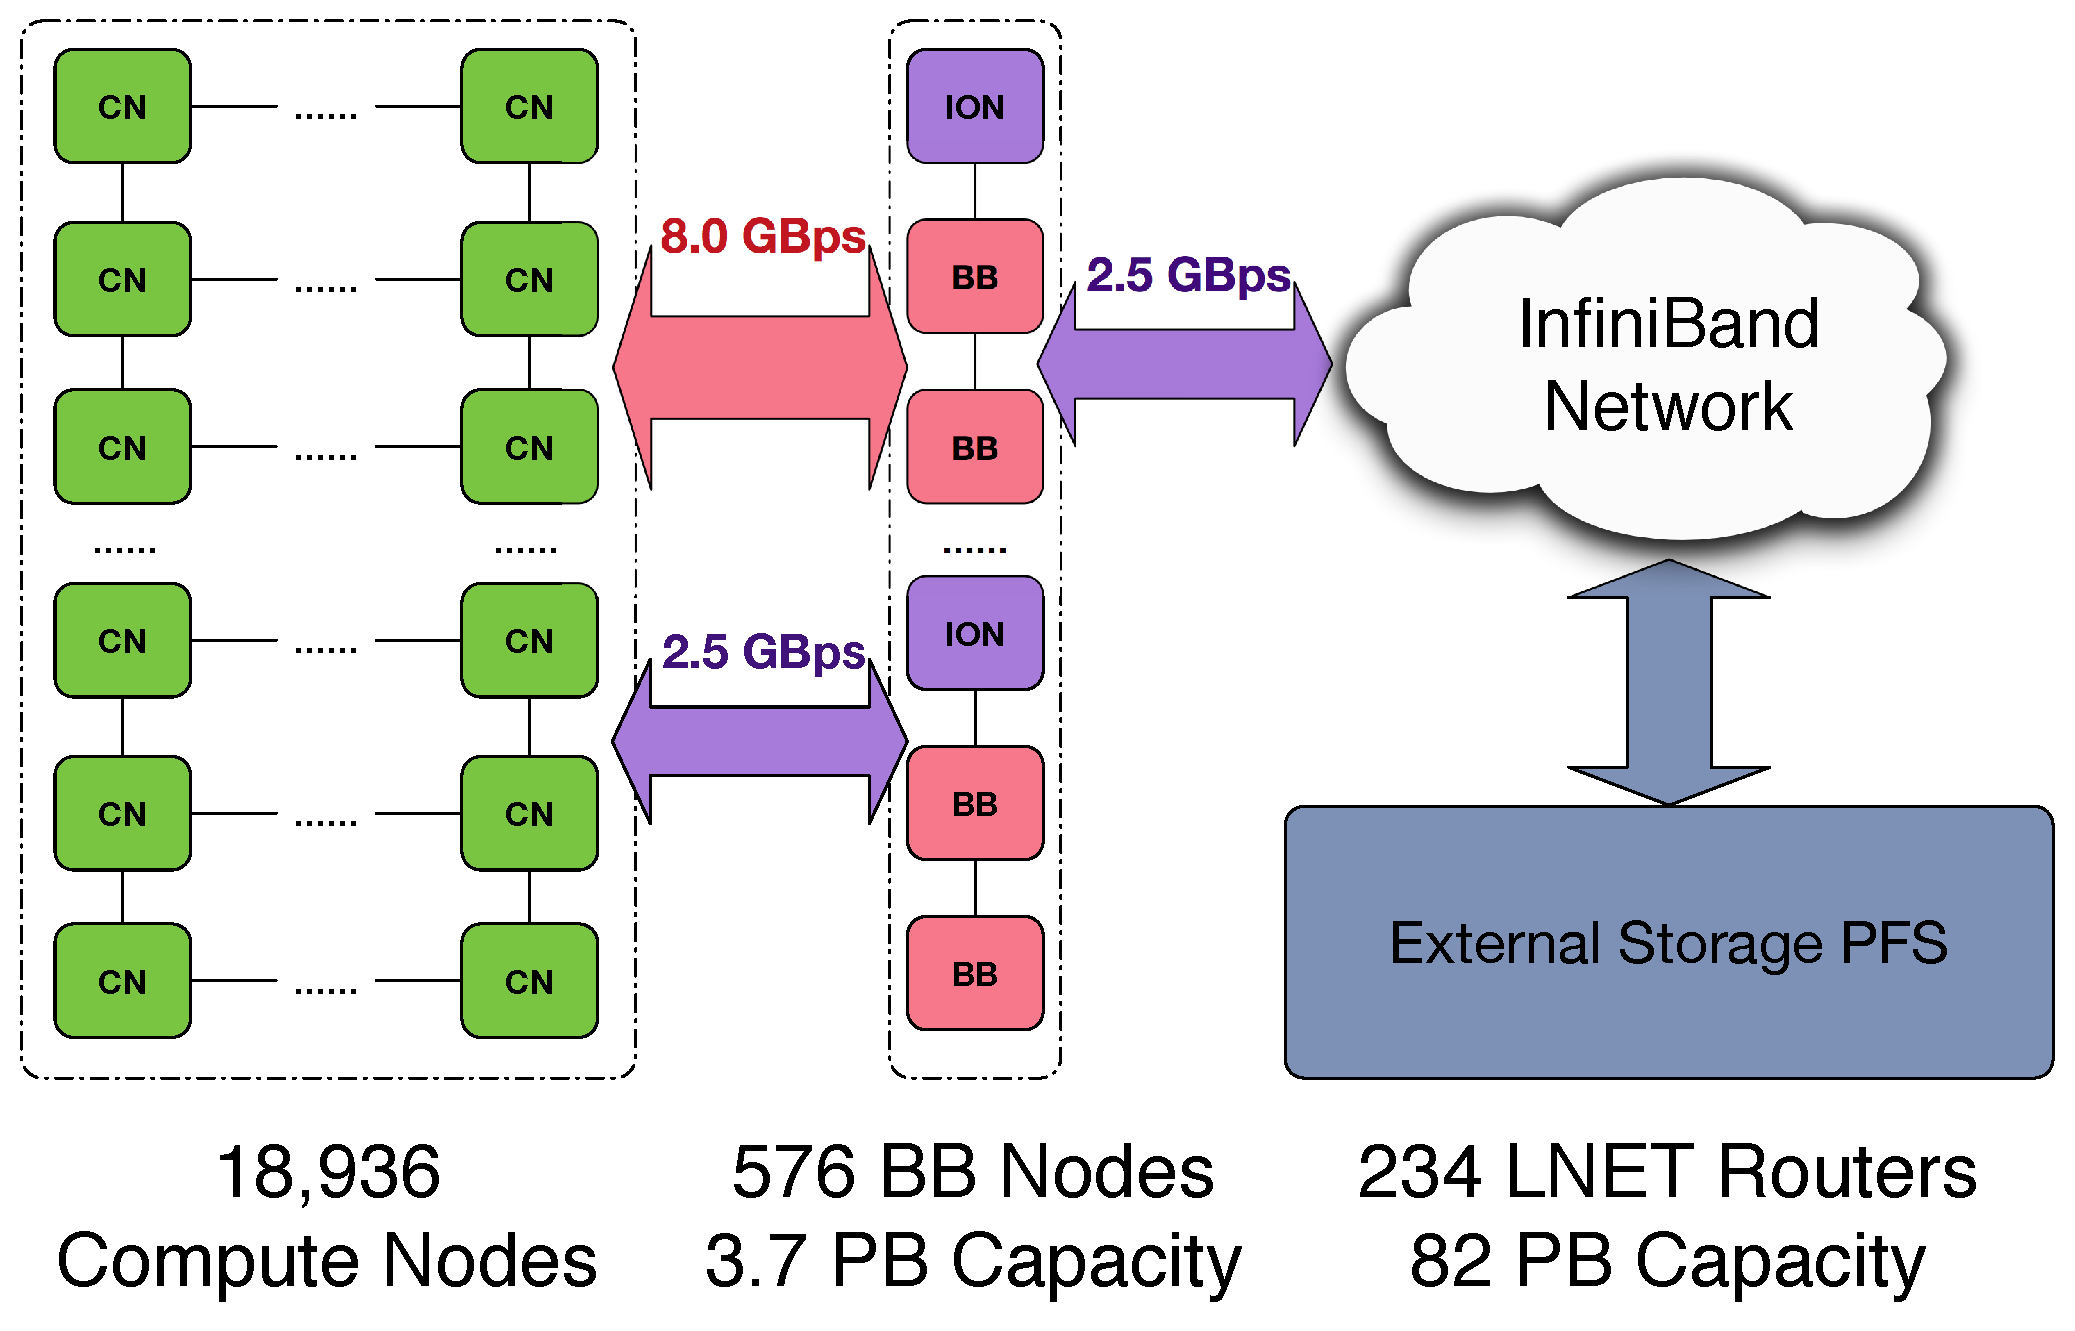
\includegraphics[width=3.5in]{BBArchitecturewithBandwidth}
        \caption{A burst buffer enabled system simulated in BBSim. The bandwidth between compute nodes and burst buffer node is 8.0 GBps (denoted by red arrow). The bandwidth between compute nodes and I/O nodes, and the bandwidth between I/O layer and the outside InfiniBand Network are set to 2.5 GBps (denoted by purple arrow).}
\label{Fig:BBArchitecture}
\end{figure}

% % trace
% Job trace is from ANL's Blue Gene Intrepid system,
% containing totally 68,936 jobs run during January to September 2009\cite{JobTrace}.
% We extract two critical fields from this jobs trace: running time and
% number of cores user requested.
% In this section we take a window of 1,185 jobs and report their scheduling results.
% We patched 3 fields to each job's log entry: the amount of input data $data\_in$,
% the total amount of written data for checkpointings $data\_run$
% and the amount of output data $data\_out$.
% We assume $data\_run$ and $data\_out$ follows uniform distribution with
% lower boundary of 1 TiB and upper boundary of 60 TiB;
% $data\_in$ follows uniform distribution between 1 GiB and 30 Gib.
% The patches 3 fields may or may not be used in scheduling,
% depends on both the model of the jobs and the experiment scenario.


\section{Experiments}
\label{Sec:Experiments}

% This section evaluate Cerberus by answering several key questions.
% \begin{itemize}
%         \item \textbf{Q1}: will Cerberus improve application performance
%                 by utilizing burst buffer nodes?
%         \item \textbf{Q2}: Will job demand on burst buffer affect Cerberus?
%                 Why bother to divide the job execution into 3 phases?
%         \item \textbf{Q3}: Can dynamic programming based optimization
%                 help Cerberus further
% improve application performance?
% \end{itemize}
% Our newly developed event-driven simulator, BBSim, is used to simulating
% the Trinity system described later.

We evaluate Cerberus through a series of experiments with BBSim.
The experimental results give answers to the following three key questions.
\begin{itemize}
        \item \textbf{Q1}: Does the use of burst buffer 
        improve both system-level and job-level performance?
%         \item \textbf{Q2}: What is the benefit of using 
%         fine-grained three-phase scheduling?
        \item \textbf{Q2}: What is the benefit of using 
        multiple queues to schedule jobs in a finer granularity than the single queuing system such as SLURM and PBS?
        \item \textbf{Q3}: What is the performance gain achieved 
        by the optimization proposed in section~\ref{SubSec:OptStageIn}-\ref{SubSec:OptStageOut}?
\end{itemize}

%traces
Our experiments are based on trace-driven simulation.
The Trinity system simulated by BBSim can be driven 
by workload trace collected from production systems.
%Since Trinity is not available to use at present, 
%there is no workload traces from Trinity available for our study.
In this paper, we use the workload trace collected from the Intrepid, a IBM Blue Gene/P system. 
The trace file contains 68,936 jobs
submitted to the system from January to September in 2009~\cite{Tang:IPDPS:2010}.
For each job, its log contains information such as submitted time, expected runtime, wait time, user ID, group ID, etc.
We patched three fields to each job's log entry: the amount of input data $data\_in$,
the total amount of written data for checkpointing $data\_run$
and the amount of output data $data\_out$.
We assume $data\_run$ and $data\_out$ follows the uniform distribution with a
lower bound of 1 TB and a upper bound of 60 TB;
$data\_in$ follows the uniform distribution between 1 GB and 30 GB~\cite{Liu:MSST:2012}.

% metric
We use three commonly used scheduling evaluation metrics,
\textit{job response time}, \textit{job waiting time} and \textit{system throughput}.
Job response time is the time duration between the job submission and its completion,
which is the major concern from user's perspective. 
Job waiting time is the aggregated wait time that a job stays in all three queues.
System throughput is defined as the number of jobs finished in
a fixed time period (500 seconds).


\subsection{Utilizing Burst Buffer Versus Direct I/O}
\label{Sec:Sim:DirectIOvsBB}

We examine the scheduling performance when 
jobs perform I/O operation in two different ways, 
namely, \textit{utilizing burst buffer} and \textit{Direct I/O}.
In the Trinity architecture, parallel file system (PFS) is mounted by all the compute nodes,
applications have the option to bypass the burst buffer 
and to use the file system directly for their I/O operations.
We refer this scenario as \textit{Direct I/O}. 
Apparently, the performance of \textit{Direct I/O}
is limited by the bandwidth of the I/O nodes. 
%However, applications will be exempted from
%waiting in the stage-in and stage-out phases in 
%the case of \textit{Direct I/O} rather than utilizing the burst buffer
%for I/O operations.


% Figure~\ref{Fig:DirectIOvsBBResponse} compares CDF of the response time of 1185 jobs.
% When scheduler can allocate burst buffer to jobs,
% response time is bounded by 376,443.12 seconds.
% However, the worst case in system without burst buffer
% (Direct IO) is catastrophical.
% There are jobs that takes 889,239.20 seconds to finish,
% which is 2.36 times slow as the most non-responsive job
% in system equipped with burst buffer.
% In average case, \textit{nearly 99\% of the jobs scheduled by Cerberus
% respond faster than Direct batch scheduler on non-BB system.}
% The improvement mainly comes from the difference of I/O operation efficiency between
% traditional I/O nodes and burst buffer nodes.

%=============XY==============
Figure~\ref{Fig:DirectIOvsBBResponse} compares CDFs of job response
time on the burst-buffer-enabled system and the traditional system (Direct I/O).
For the burst-buffer-enabled system, the job response time is bounded by 376,443.12 seconds.
However, the worst case of Direct I/O is catastrophic, 
i.e., a job takes 889,239.20 seconds to finish,
which is 2.36 times slower than the slowest non-responsive job
in the burst-buffer-enabled system.
In average, \textit{nearly 99\%} of the jobs scheduled on the burst-buffer-enabled system
respond faster than the traditional system without burst buffer, since the burst buffer can mitigate the I/O gap between I/O nodes and compute nodes.


% Figure~\ref{Fig:DirectIOvsBBWait} reveals the total waiting time for both cases.
% Notice that system without burst buffer only request compute nodes.
% In this case, waiting time is the duration from its submission
% to actual starting running.
% The difference of worst case waiting time is drastic.
% Without burst buffer nodes, job's wait duration in worst case is 3.02 times
% slow as the worst one on systems with burst buffer;
% the upper bound of waiting duration for burst buffer systems is about 285,254 seconds.
% Because of burst buffer's better ability to
% absorb checkpoint operations and data moving in/out,
% the execution pipeline of job series is significantly speed up.
% Statistically, \textit{more than 80\% jobs waited less time, thus respond faster,
% if they can access burst buffer.}

%=============XY==============
Figure~\ref{Fig:DirectIOvsBBWait} reveals the aggregated job waiting time.
Note that in the case of Direct I/O, jobs only request compute nodes.
Thus, the waiting time is the duration between the job submission and the job starting time.
The difference of the worst case waiting time in the both systems is drastic.
On the system without burst buffer nodes, the waiting duration in the worst case is 3.02 times
slower than the worst case in the burst-buffer-enabled system.
The upper bound of the waiting duration for the burst buffer systems is about 285,254 seconds.
Because burst buffer has better ability to absorb checkpoint operations and data moving in/out,
the execution pipeline of job series is significantly fast.
Statistically, \textit{more than 80\% jobs have less waiting time if they utilize burst buffer.}

% Using the collected completion time, we calculate system's throughput over time sequence.
% Figure~\ref{Fig:DirectIOvsBBThroughput} shows the system throughput for
% both system using burst buffer nodes and not.
% As indicated by the bar chart,
% \textit{the ratio of average throughput between two systems is 2.36},
% namely 1.575 to 0.667.
% It totally takes 889,239 seconds for the system without burst buffer nodes to
% server all 1185 jobs.
% The last job is job \#1150, which requested 4096 cores and 59 TB data space.
% It starts at 1126 seconds but waited 827,241 seconds.
% In contrast, when system installed burst buffer nodes,
% it accomplishes the same 1185 jobs in 376,443 seconds.
% Job \#1150 is the second last job finished, but both its waiting time and response time
% are significantly reduced, 272,741 and 376,026 seconds respectively.

%=============XY==============
Figure~\ref{Fig:DirectIOvsBBThroughput} shows the system throughputs.
As indicated by the bar chart, \textit{the ratio of the average throughput between the two systems is 2.36}, i.e.,1.575 to 0.667.
It takes 889,239 seconds for the system without burst buffer nodes to
complete the workload. We pick a specific job with ID \#1150 from the workload, and observe its
waiting time in both cases.
Job \#1150 requested 256 compute nodes and 59 TB data space.
It started in the 1,126 second, but waited for 827,241 seconds.
In contrast, for the burst-buffer-enabled system, the same job accomplished the same workload in 376,443 seconds, and the waiting time and the response time of job \#1150
are significantly reduced, i.e., 272,741 and 376,026 seconds respectively.


\begin{figure*}[t]
        \centering
        \subfloat[Job Response Time] {
                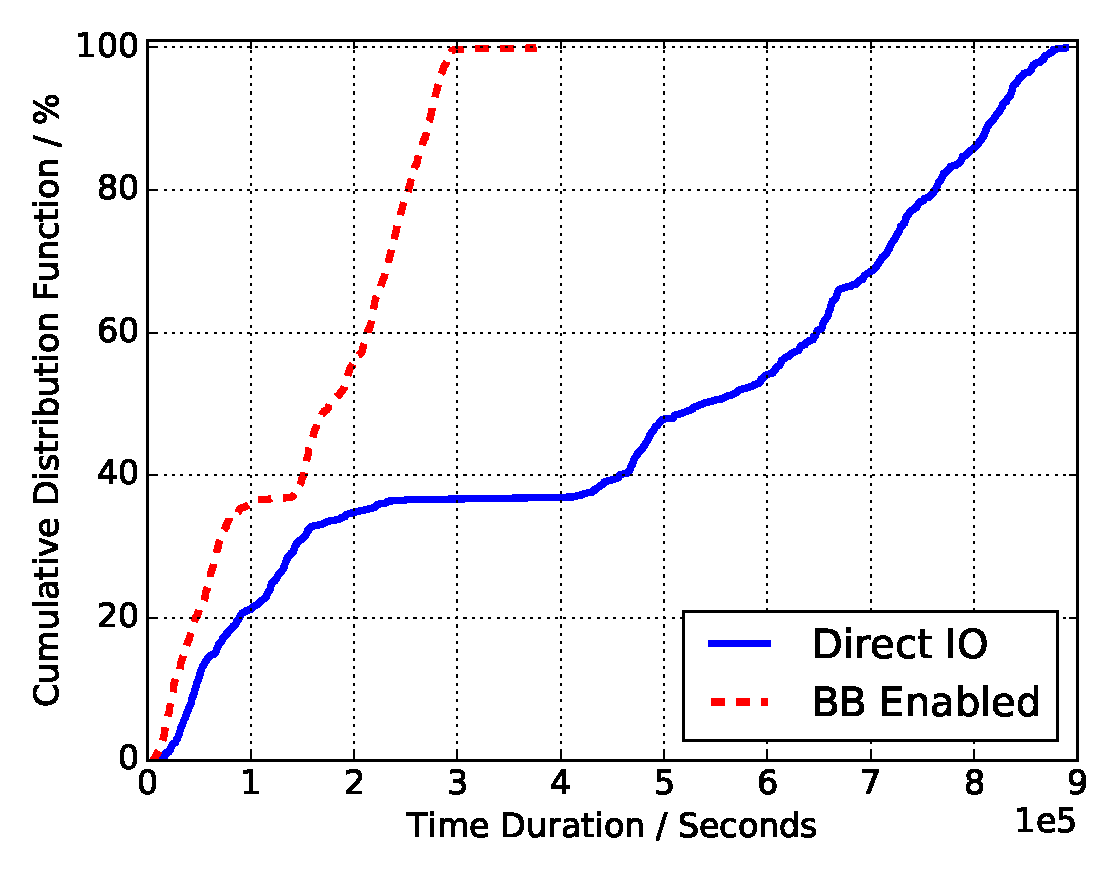
\includegraphics[width=2.2in]{IOvsBBFigures/1000jobs_direct_vs_bb_response}
                \label{Fig:DirectIOvsBBResponse}
        }
        \subfloat[Job Aggregated Wait Time] {
                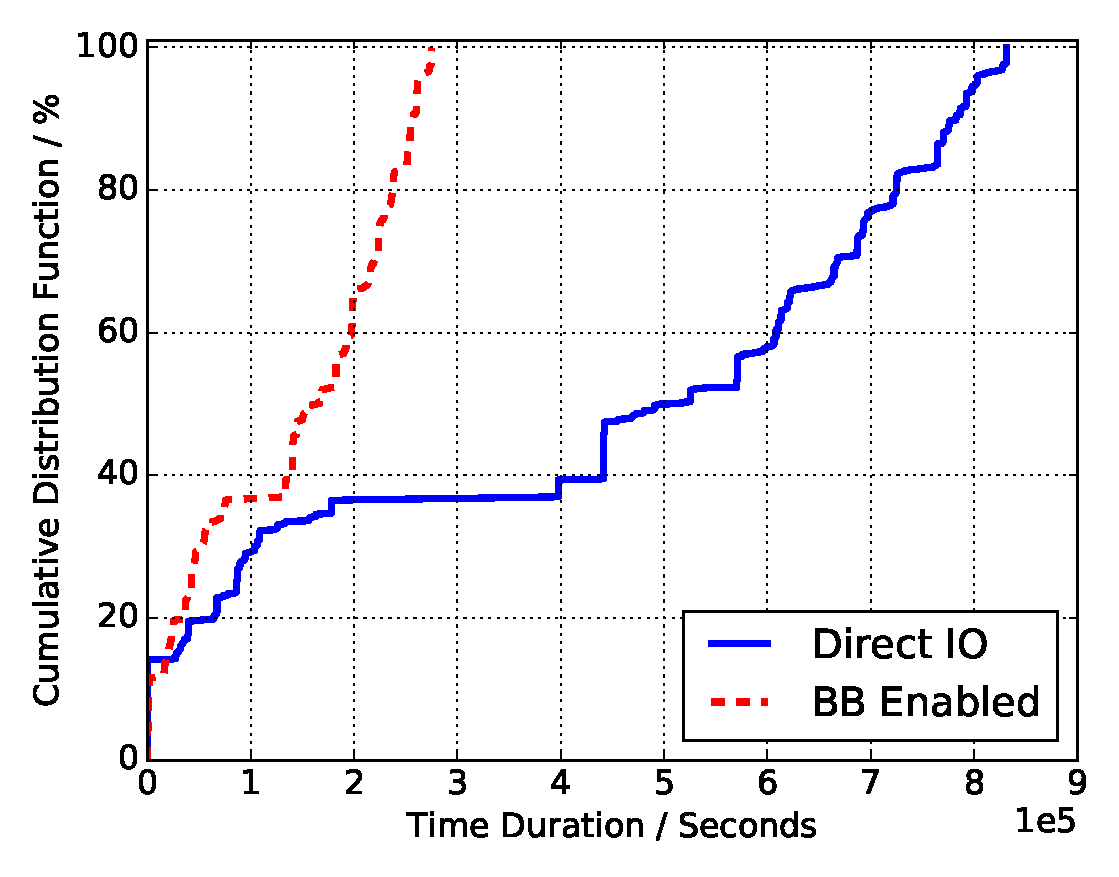
\includegraphics[width=2.2in]{IOvsBBFigures/1000jobs_direct_vs_bb_wait}
                \label{Fig:DirectIOvsBBWait}
        }
        \subfloat[System Throughput] {
                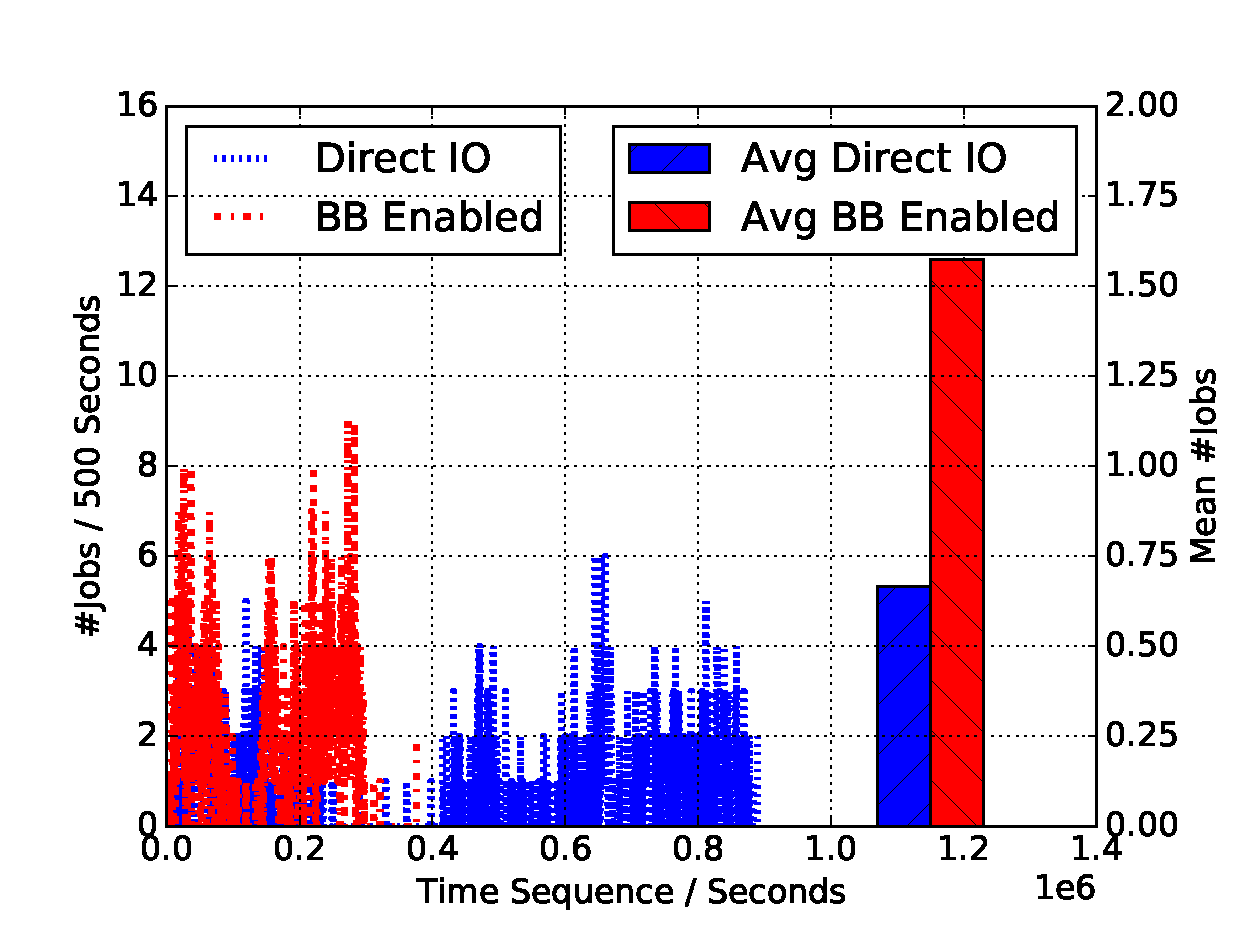
\includegraphics[width=2.5in]{IOvsBBFigures/1000jobs_direct_vs_bb_throughput}
                \label{Fig:DirectIOvsBBThroughput}
        }
        \caption{The comparison of scheduling performance between job utilizing burst buffer and conducting Direct I/O. In (c), on the left, the system throughput is presented in time sequence; the average system throughput is presented on the right. }
        \label{Fig:DirectIOPerformance}
\end{figure*}

%\begin{figure}[!t]
        %\centering
        %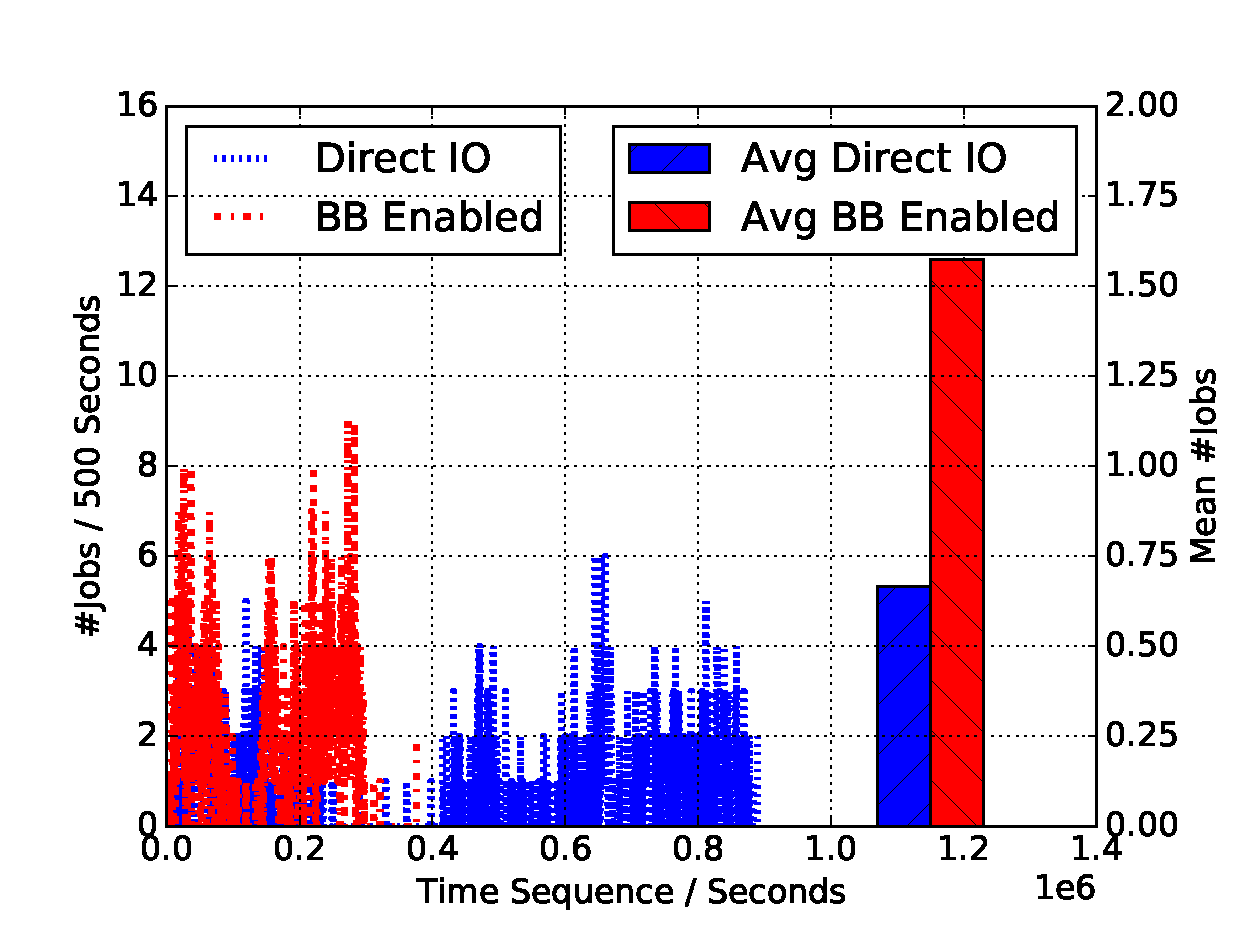
\includegraphics[width=3.2in]{IOvsBBFigures/1000jobs_direct_vs_bb_throughput}
        %\caption{System Throughput, IO Node Only vs. Burst Buffer System}
        %\label{Fig:DirectIOvsBBThroughput}
%\end{figure}
In short, the above experiments allow us to answer Q1.
That is, \textit{the use of burst buffer can improve both system-level and job-level performance.}
%Based on the above comparison, we can answer question \textbf{Q1}: 
%by utilizing burst buffer nodes,
%both the job-level and system-level performance can be significantly improved.
\textit{The execution of 99\% jobs will be expedited, 
80\% of jobs will suffer less wait time,
and the average system throughput will be improved as much as 136\%.}




\subsection{Three-Phase Model Versus One-Phase Model}

% In Figure~\ref{Fig:3Pvs1PResponse}, we plot 3 different scheduling results by 3 FCFS scheduler.
% \begin{itemize}
%         \item \textbf{1-Phase BB}: Jobs are modeled as just 1 phase.
%                 Users just provide general burst buffer demand throughout
%                 entire application lifetime.
%         \item \textbf{1D Cerberus}: In this case Cerberus only knows
%                 the overall burst buffer demand.
%         \item \textbf{Cerberus}: Users kindly provided all the burst buffer
%                 demand in all 3 phases.
%                 %the same as Cerberus in section~\ref{Sec:Sim:DirectIOvsBB}
% \end{itemize}
% We simulate the 3 cases with the same generated random data volume sequence.
% We assume the overall burst buffer demand in 1-phase BB and 1D Cerberus is
% $\max \{data\_in, data\_out, data\_run\}$.
% Notice that 1-phase BB scheduler must subject to burst buffer capacity constraint.
% %For 1-phase-modeled jobs, scheduler will make decision
% %based on $\max \{data\_in, data\_out, data\_run\}$
% %since we assume user will only tell the upper bound of its application's demand.
% %However, in simulation, we use the generated data amount as the same as 3-modeled jobs.
% %Response time of system without burst buffer devices are also plotted for comparison.

%========XY========================
We investigate the performance of scheduling jobs in different models. 
As we discussed before, Cerberus is designed for scheduling the three-phase modeled jobs. 
It makes scheduling decisions in fine granularity. 
In Figure~\ref{Fig:3Pvs1PResponse}, the scheduling results based on three job models
are presented:
\begin{itemize}
        \item \textbf{1-Phase-1D}: Jobs are submitted with the total burst buffer demand,
        but their lifetime are not divided into three phases. 
	Instead, the scheduler makes scheduling decision only once for each job.

        \item \textbf{3-Phase-1D}: Jobs are submitted with the total burst buffer demand,
        their lifetime are divided into three phases as discussed in Section~\ref{Sec:Model}.
        
        \item \textbf{3-Phase-3D}: Jobs are submitted with the detailed burst buffer demand in each phase.

\end{itemize}
We assume the overall burst buffer demand in 1-Phase-1D and 3-Phase-1D is
$\max \{data\_in, data\_out, data\_run\}$.
Notice that 1-phase BB scheduler must subject to the burst buffer capacity constraint.
Cerberus is responsible for scheduling jobs in 3-Phase-1D and 3-Phase-3D model.
The scheduling policy used in this experiment is first-come first-serve.

% 
% %Unsurprisingly, jobs' response time is improving as long as they could utilizing burst buffer.
% When comparing scheduling results of 1-Phase BB and 1D Cerberus,
% both of which only have rough data information of application,
% more than 60\% of the 3-phase-modeled jobs finish faster than 1-phase-modeled jobs.
% The longest 3-phase-modeled job takes 418,927 seconds to finish
% while the slowest 1-phase-modeled job needs about 492,591 seconds to finish.
% The improvement is about 14.95\% for the worst case.
% The reason of such improvement is as follows.
% For the 1-phase-modeled jobs, burst buffer nodes will be exclusively
% taken by scheduled jobs throughout their lifetime.
% In contrast, Cerberus will reclaim burst buffer multiple times;
% it also releases burst buffer nodes and CPU resources as soon as possible.
% This gives Cerberus more opportunity to schedule the system resources.
% At last, when comparing the case of Cerberus with 1D Cerberus,
% we find another advantage of our 3-phase model.
% If benign users can provide finer-grain information of data/I/O demand,
% Cerberus can programme each queue separately and get better scheduling result.
% In our simulation,
% since Cerberus knows more about application's demand in different phases,
% the worst absolute response time is less than 379,026 seconds.
% This is 10.24\% improvement to 3-phase-modeled jobs
% when Cerberus only knows the upper bound of data demand,
% 23.66\% better than the slowest 1-phase-modeled job.
% In average case, \textit{more than 80\% of the jobs 
% scheduled by Cerberus finish earlier than 1-phase-modeled jobs.}
% Meanwhile, \textit{more than 60\% of the jobs takes less time if user 
% specifies data usage demand at each phase to Cerberus, e.g. Cerberus vs. 3-Phase-1D.}


%==============XY===============
When comparing the scheduling results of 1-Phase-1D and 3-Phase-1D,
both of which only have the overall burst buffer demand of each job,
more than 60\% of the three-phase-modeled jobs finish faster than the 1-phase-modeled jobs.
The slowest three-phase-modeled job takes 418,927 seconds to finish,
while the slowest 1-phase-modeled job takes about 492,591 seconds to finish.
The improvement is about 14.95\% in the worst case scenario.
Here is the explanation: For the 1-phase-modeled jobs, the burst buffer nodes will be exclusively
taken by the scheduled jobs throughout their lifetime. In contrast, Cerberus reclaims the burst buffer multiple times;
It also releases the burst buffer nodes and the CPU resources at the earliest possible time, which allows Cerberus to schedule more system resources.
%Finally, when comparing the cases of 3-Phase-3D with 3-Phase-1D, we find another advantage of our 3-phase model.
In addition, if users can provide fine-grain information of data I/O demands,
Cerberus can coordinate three queues and make scheduling decision separately to achieve better scheduling result.
For the 3-Phase-3D model, Cerberus knows each job's demand during the different phases,
the worst absolute response time is less than 379,026 seconds.
This is about 10.24\% improvement to three-phase-modeled jobs.
When Cerberus only knows the upper bound of data demand,
it is 23.66\% better than the slowest 1-phase-modeled job.
In average, \textit{more than 80\% of the three-phase-modeled jobs
finish earlier than 1-phase-modeled jobs.}
Meanwhile, \textit{more than 60\% of the jobs take less time if user
specifies data usage demand at each phase, e.g., 3-Phase-3D vs. 3-Phase-1D.}



% We can reason about why Cerberus's scheduling result is better than
% naively integrating batch scheduler with burst buffer constraint
% by looking at the detailed waiting time.
% Figure~\ref{Fig:3Pvs1PWaitRun} shows the time job spend in running queue.
% There are 3 queues in Cerberus;
% correspondingly we have 3 kinds of waiting for jobs in Cerberus.
% %Figure~\ref{Fig:3Pvs1PWaitIn} shows the time job spend in inputing queue,
% %Figure~\ref{Fig:3Pvs1PWaitOut} the time job spend in outputing queue.
% For 1-phase-modeled jobs, there is just one queue;
% therefore the waiting time in Figure~\ref{Fig:3Pvs1PWaitRun} is the total waiting time.
% We see that jobs did not spend much time in either input queue $Q_I$ or output queue.
% The upper bounds of time spent in input queue are
% 2500 seconds for 1D Cerberus and Cerberus respectively.
% This is because input data is very small (tens of GB level)
% comparing to checkpointing data and application output (tens of TB level).
% In contrast, in worst case job scheduled by 1-Phase BB needs to wait for 443,203 seconds,
% because scheduler makes one-time decision on the basis of demand of
% both computer node and maximum burst buffer.
% %the upper bounds of time spent in output queue $Q_O$ are
% %less than 5\% of the total waiting time of 1-phase-scheduler case
% %for both 3-phases cases.
% As for the time waiting for running, more than 60\% of the jobs scheduled by
% 1D Cerberus and Cerberus are better than 1-phase-modeled jobs.
% The difference of waiting time results in the different
% response performance.


We now investigate the detailed waiting time to understand why the scheduling results in Cerberus
are better than the naive integration of the batch scheduler with the burst buffer constraints.
Figure~\ref{Fig:3Pvs1PWaitRun} shows the waiting running time, how long a job spent in the running queue.
There are three queues in Cerberus.
Correspondingly jobs in Cerberus have three kinds of waiting time: waiting input, waiting running, and waiting output time.
%Figure~\ref{Fig:3Pvs1PWaitIn} shows the time job spend in inputing queue,
%Figure~\ref{Fig:3Pvs1PWaitOut} the time job spend in outputing queue.
For 1-phase-modeled jobs, there is just one queue.
Therefore, the waiting time in Figure~\ref{Fig:3Pvs1PWaitRun} is the total waiting time.
We observe that (not shown in Figure~\ref{Fig:3Pvs1PWaitRun}) the jobs did not
take much time either in the input queue $Q_I$ nor in the output queue.
The upper bounds of time spent in the input queue, e.g. waiting time in $Q_I$, are 
2,500 seconds for both 3-Phase-1D and 3-Phase-3D modeled jobs.
This is because that the input data are very small (e.g., tens of GB)
compared to the checkpointing data and the application output (e.g., tens of TB).
In contrast, in the worst case of 1-Phase-1D, the job waiting time is 443,203 seconds,
because the scheduler makes a one-time decision based on the demand of the computer node and the maximum burst buffer.
%the upper bounds of time spent in output queue $Q_O$ are
%less than 5\% of the total waiting time of 1-phase-scheduler case
%for both 3-phases cases.
As for the time waiting for running, more than 60\% of the 3-Phase-1D and 3-Phase-3D modeled jobs are scheduled,
which is much better than the 1-phase-model.
The differences of the waiting time lead to the difference in response performance.


% Figure~\ref{Fig:3Pvs1PThroughput} describes system throughput of these three different scenarios.
% It helps us examine the performance of the scheduling in time sequence.
% For 1-phase-modeled job, we can see an obvious `throughput gap'
% from 150,000 second to 200,000 second approximately,
% similar for the case of 1D Cerberus, throughput also starts provocatively,
% Cerberus' runs counter to both previous cases.
% Even though there is a throughput trough between 100,000 to 150,000 seconds,
% Cerberus manages to make the system having high throughput at the beginning and
% later (from 150,000 to 300,000 seconds).
% \textit{In average, the throughput of Cerberus is 1.575 jobs / 500 seconds.}
% It is 11.39\% of the 1-Phase BB case (1.414 jobs / 500 seconds) and
% 31.03\% higher than the 1D Cerberus case (1.202 jobs / 500 seconds).
% We believe this validates the indispensable 3 phase job model and
% the necessity that user provides data capacity demand for each phase.

Figure~\ref{Fig:3Pvs1PThroughput} describes the system throughputs of the three different job models.
It helps us to examine the scheduling performance in a time sequence.
For 1-Phase-1D modeled job, we can see an obvious `throughput gap'
from 150,000 seconds to 200,000 seconds approximately.
The case of 3-Phase-1D Cerberus is similar.
3-Phase-3D runs counter to both previous cases.
Even though there is a throughput between 100,000 to 150,000 seconds,
the 3-Phase-3D model manages to make the system having a high throughput at the beginning and
later changes from 150,000 to 300,000 seconds.
\textit{In average, the throughput of the 3-Phase-3D model is 1.575 jobs / 500 seconds.}
It is 11.39\% higher than the 3-Phase-1D case (1.414 jobs / 500 seconds) and
23.68\% higher than the 1-Phase-1D case (1.202 jobs / 500 seconds).
We believe that the results validate the indispensable 3 phase job model and
justifies the necessity that a user needs to provide data capacity demand for each phase.



\begin{figure*}[t]
        \centering
        \subfloat[Job Response Time] {
                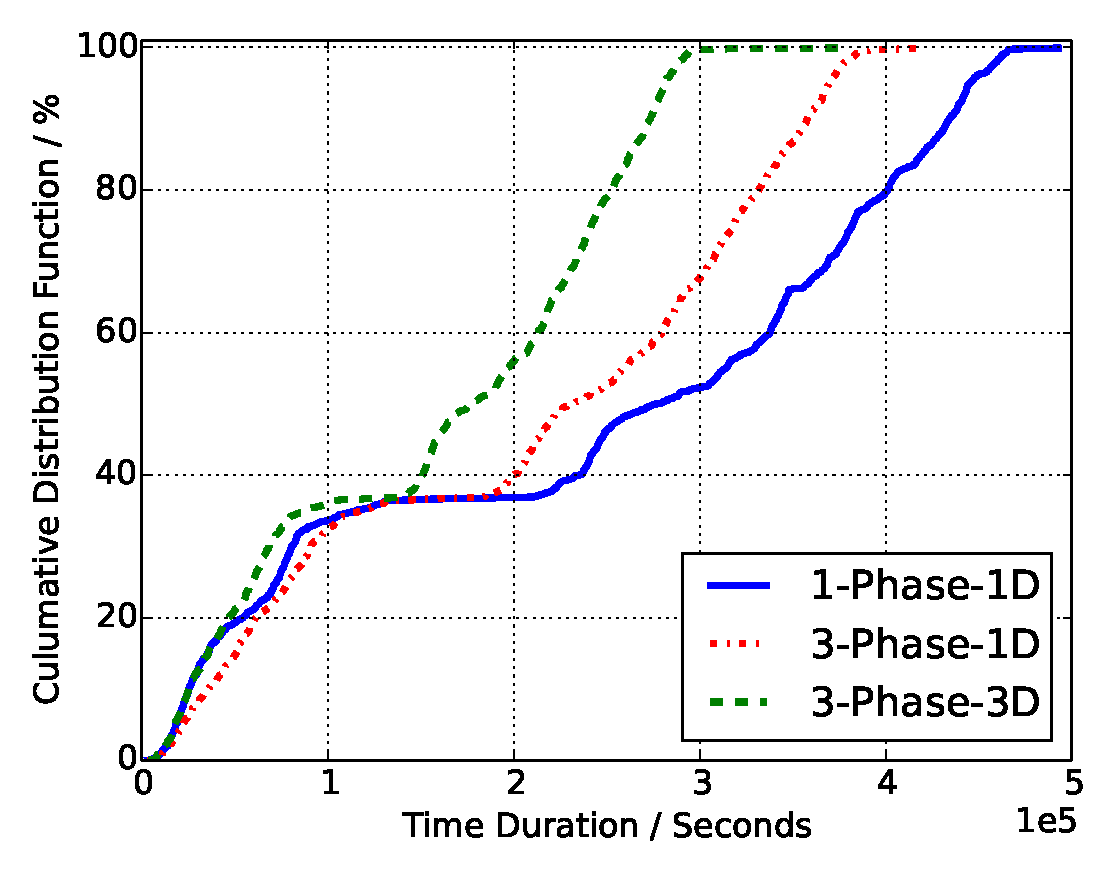
\includegraphics[width=2.2in]{3Pvs1PFigures/1000jobs_3p_vs_1p_response}
                \label{Fig:3Pvs1PResponse}
        }
        %\subfloat[Job Wait Time] {
                %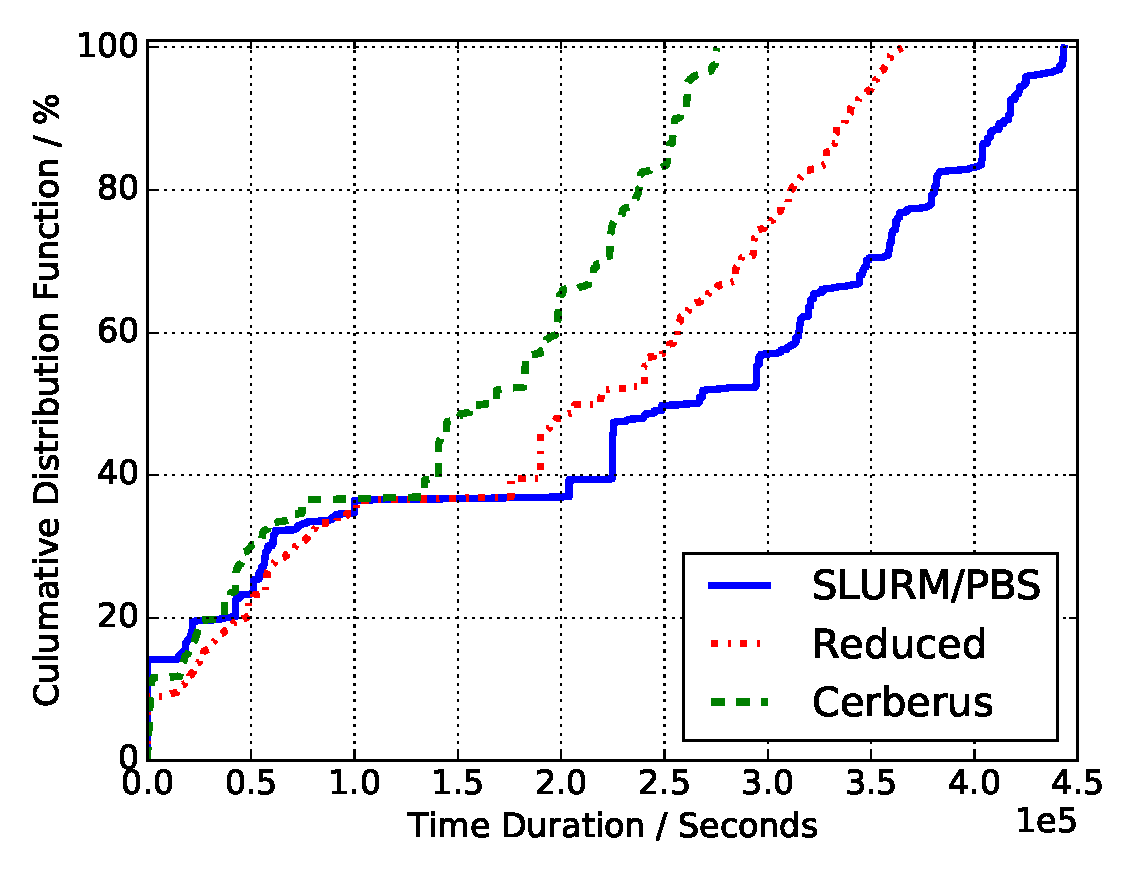
\includegraphics[width=3.2in]{3Pvs1PFigures/1000jobs_3p_vs_1p_wait}
                %\label{Fig:3Pvs1PWait}
        %}
        %\subfloat[Job Wait Input Time] {
                %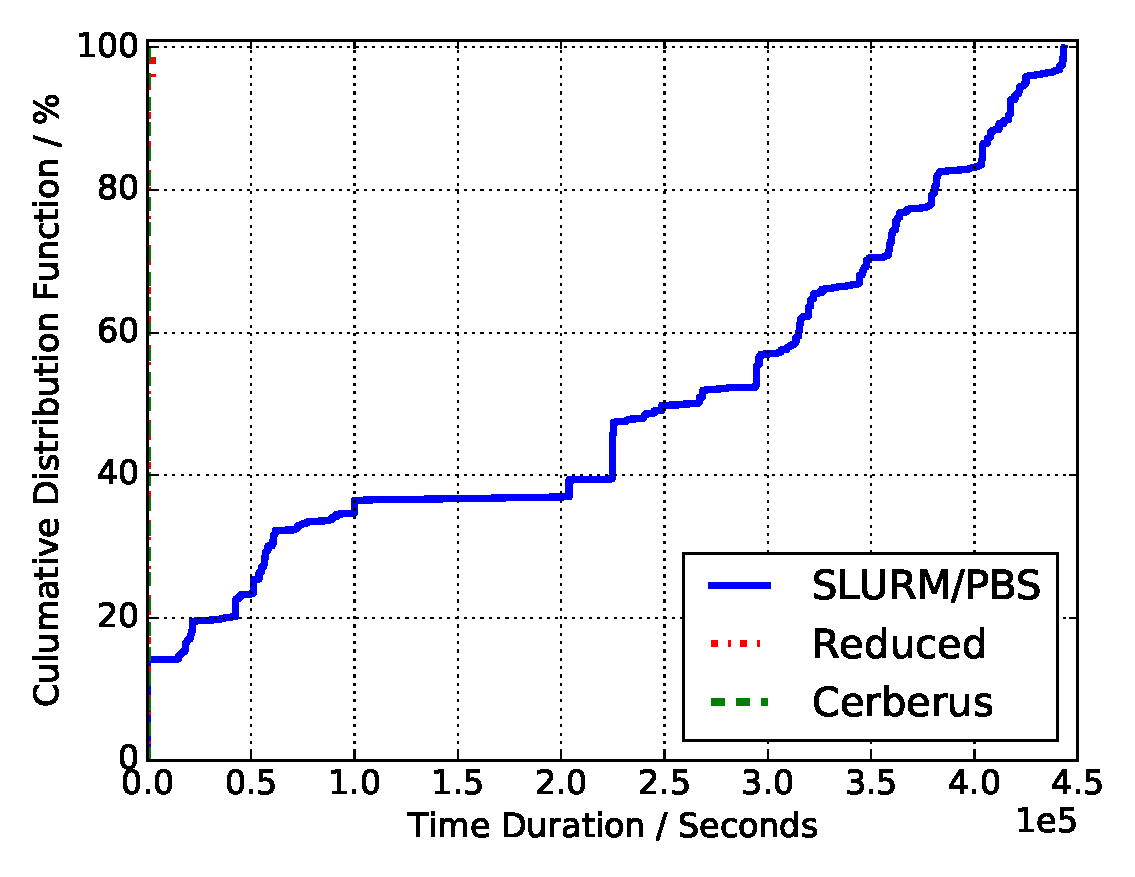
\includegraphics[width=2.3in]{3Pvs1PFigures/1000jobs_3p_vs_1p_wait_in}
                %\label{Fig:3Pvs1PWaitIn}
        %}
        %~
        \subfloat[Job Waiting Time in $Q_R$] {
                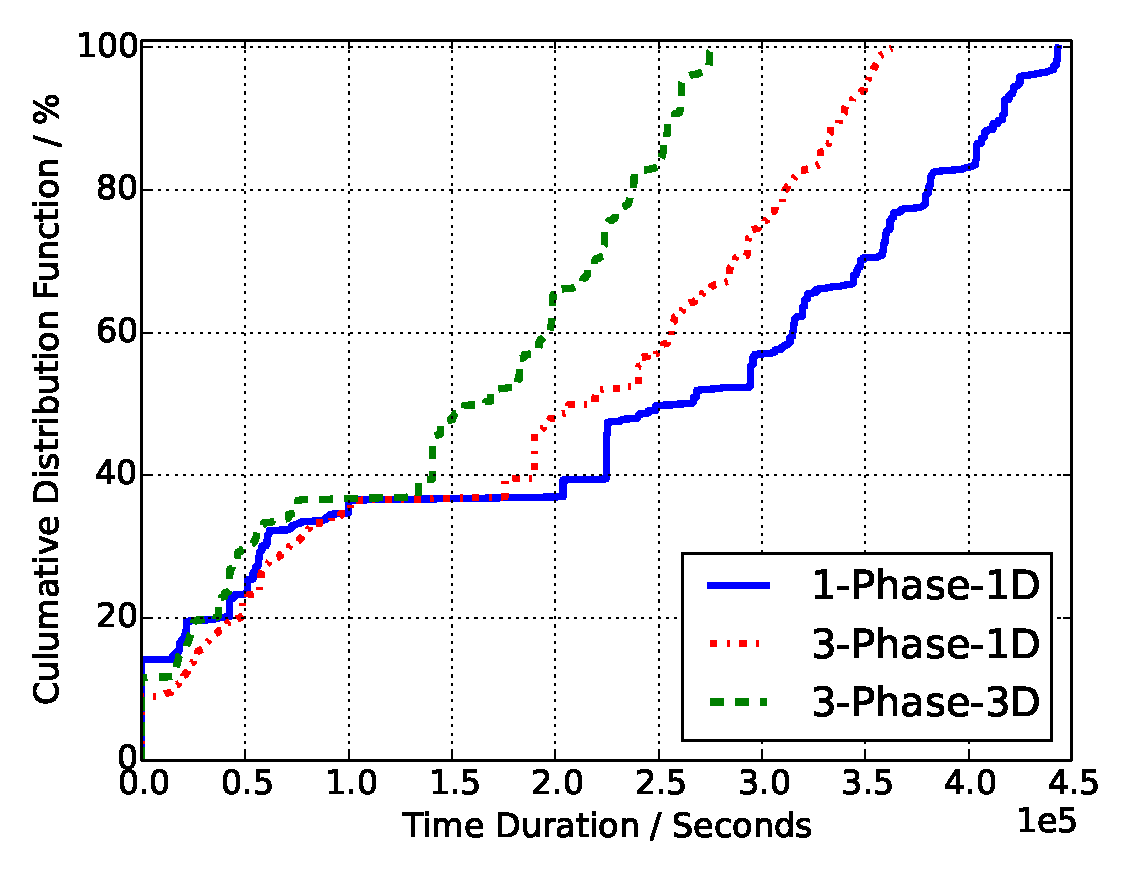
\includegraphics[width=2.2in]{3Pvs1PFigures/1000jobs_3p_vs_1p_wait_run}
                \label{Fig:3Pvs1PWaitRun}
        }
        \subfloat[System Throughput] {
                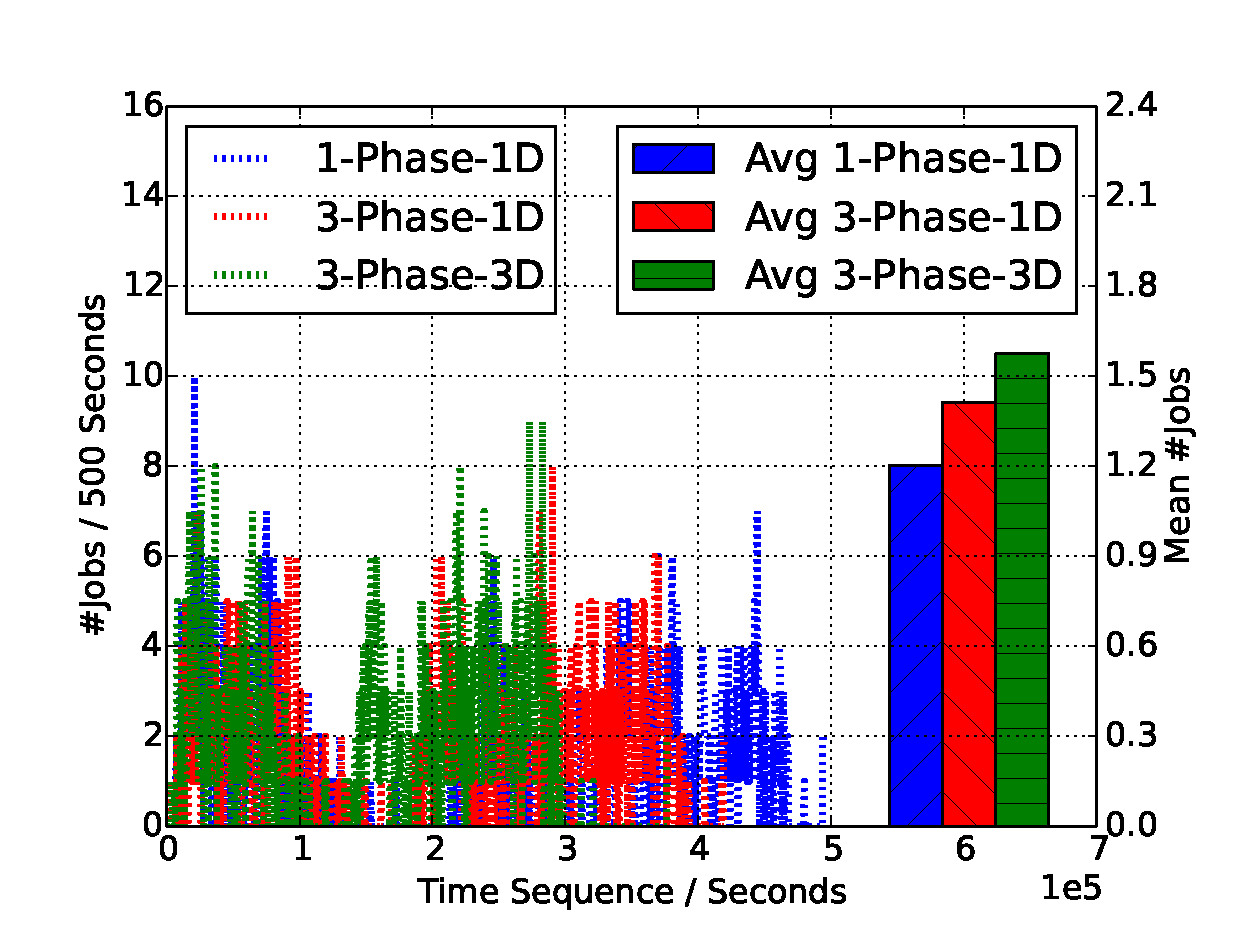
\includegraphics[width=2.5in]{3Pvs1PFigures/1000jobs_3p_vs_1p_throughput}
                \label{Fig:3Pvs1PThroughput}
        }
        \caption{The comparison of scheduling performance between using 3-phase model and 1-phase model. In (c), on the left, the system throughput is presented in time sequence; the average system throughput is presented on the right.}
        \label{Fig:3Pvs1PPerformance}
\end{figure*}

%\begin{figure}[!t]
        %\centering
        %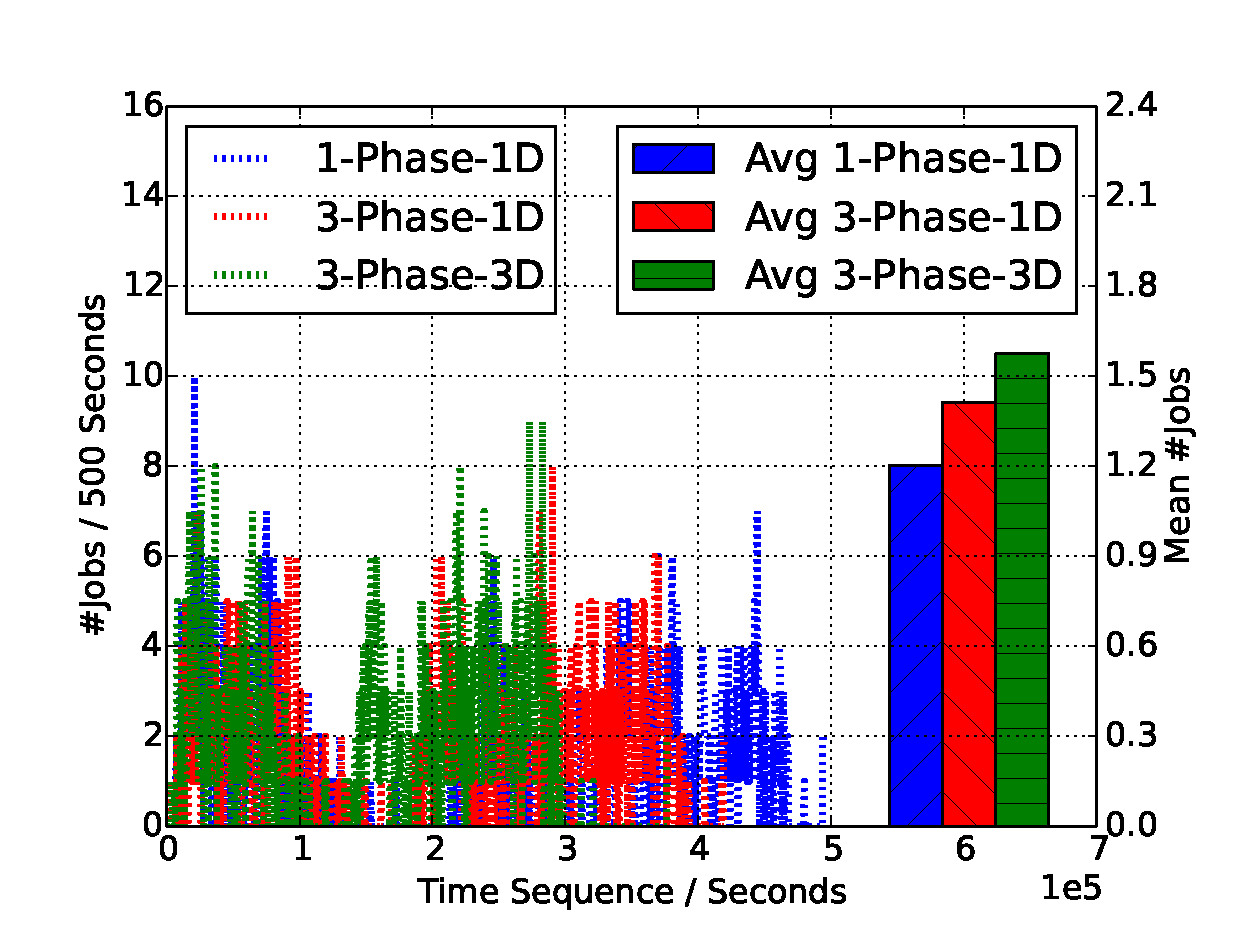
\includegraphics[width=3.2in]{3Pvs1PFigures/1000jobs_3p_vs_1p_throughput}
        %\caption{System Throughput, 1 Phase Model vs. 3 Phase Model}
        %\label{Fig:3Pvs1PThroughput}
%\end{figure}

\begin{figure*}[t]
        \centering
        \subfloat[Job Response Time] {
                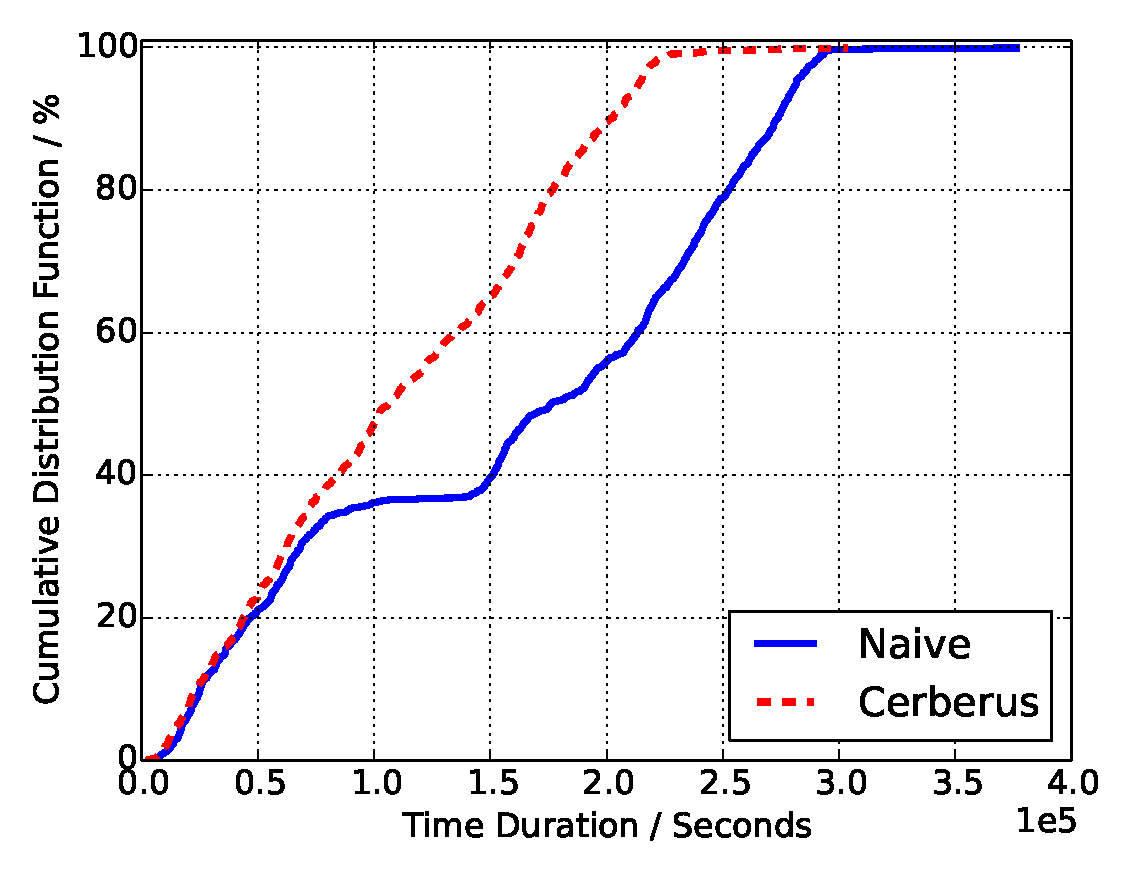
\includegraphics[width=2.2in]{DPvsFIFOFigures/1000jobs_dp_vs_fifo_response}
                \label{Fig:DPvsFIFOResponse}
        }
        \subfloat[Job Aggregated Waiting Time in $Q_R$] {
                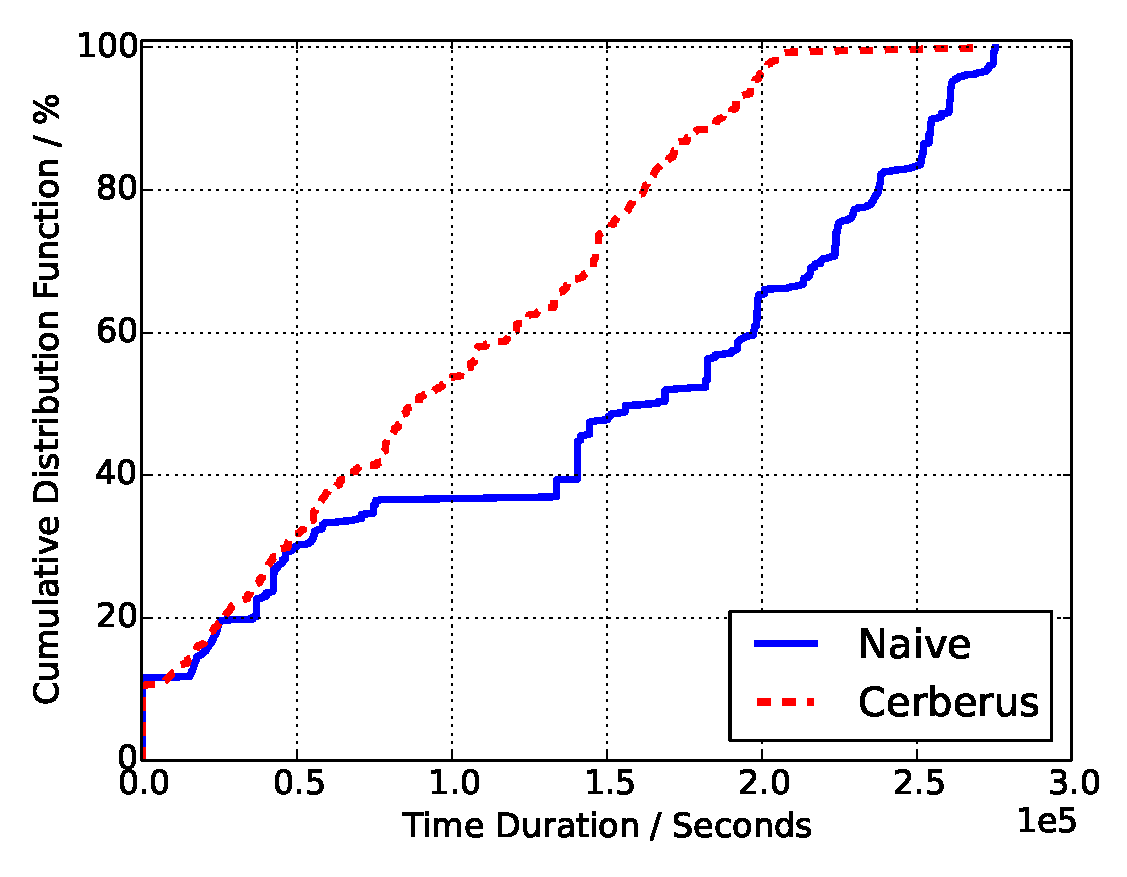
\includegraphics[width=2.2in]{DPvsFIFOFigures/1000jobs_dp_vs_fifo_wait_run}
                \label{Fig:DPvsFIFOWaitRun}
        }
        \subfloat[System Throughput] {
                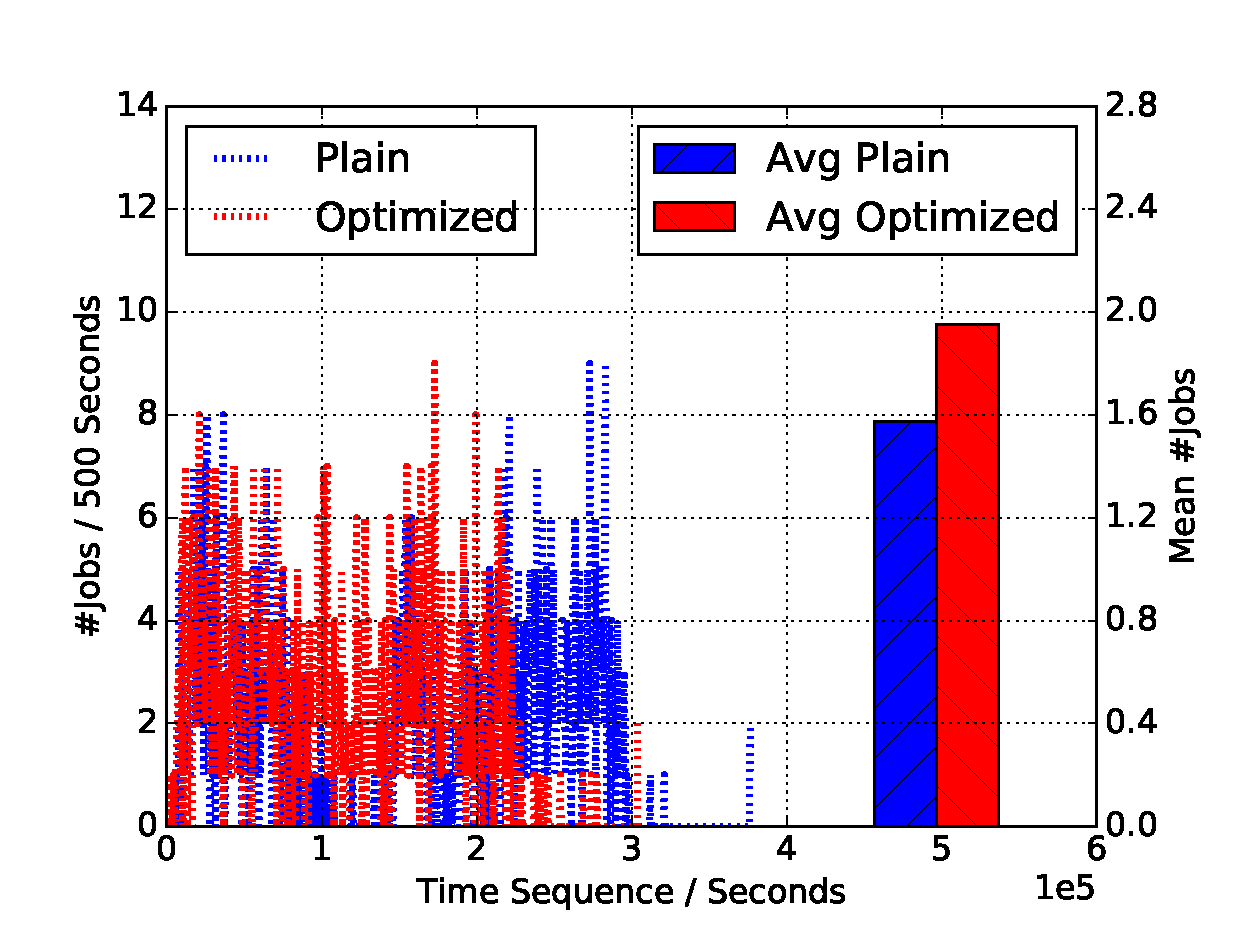
\includegraphics[width=2.5in]{DPvsFIFOFigures/1000jobs_dp_vs_fifo_throughput}
                \label{Fig:DPvsFIFOThroughput}
        }
        \caption{The comparison of scheduling performance obtained by Cerberus and a naive first-come, first-serve scheduling. In (c), on the left, the system throughput is presented in time sequence; the average system throughput is presented on the right.}
        \label{Fig:DPvsFIFOPerformance}
\end{figure*}

%\begin{figure}[!t]
        %\centering
        %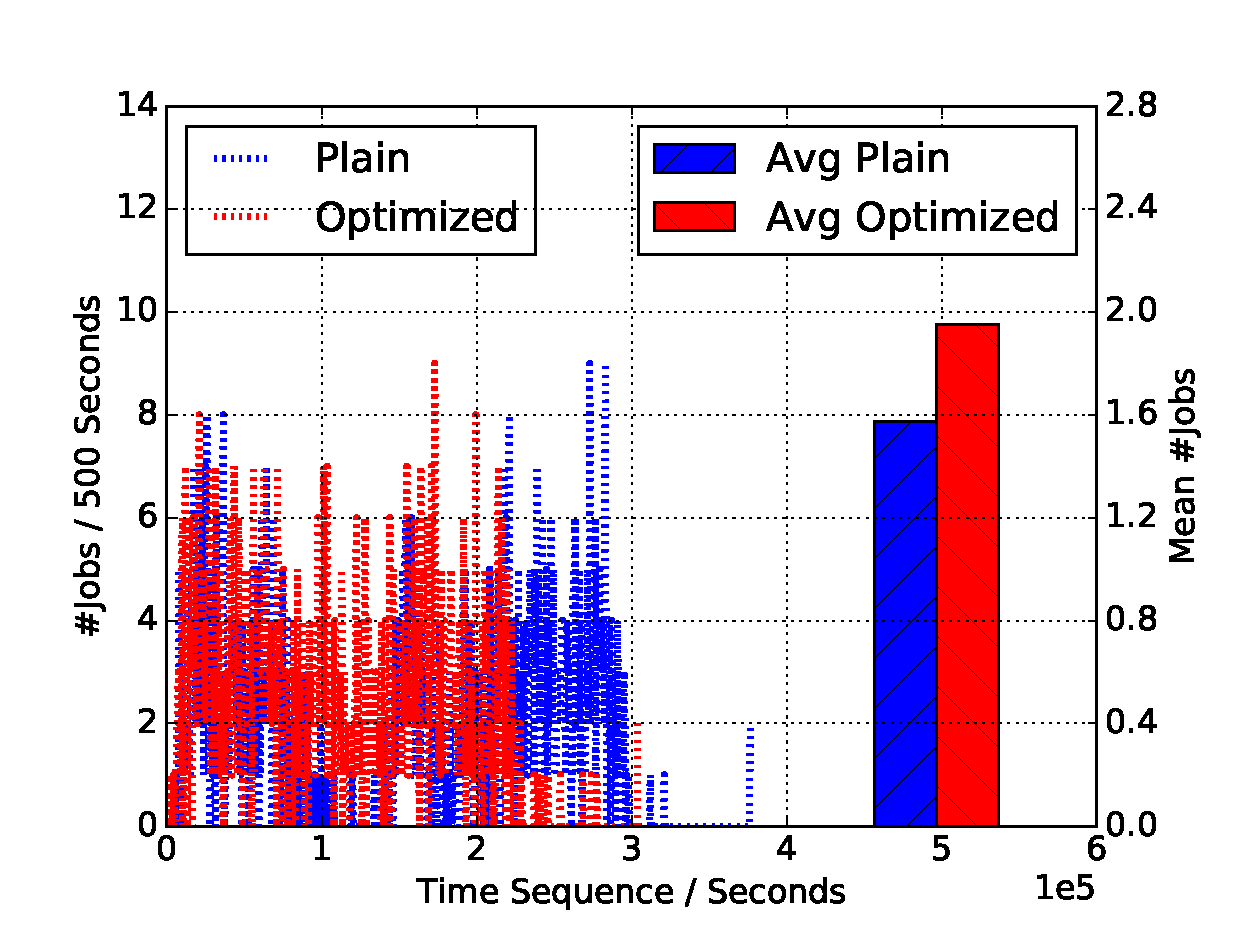
\includegraphics[width=3.2in]{DPvsFIFOFigures/1000jobs_dp_vs_fifo_throughput}
        %\caption{System Throughput, Optimized Cerberus vs. FCFS Cerberus}
        %\label{Fig:DPvsFIFOThroughput}
%\end{figure}

The experimental results demonstrate that the performance of both jobs and the system is improved 
when Cerberus makes fine granularity scheduling decisions for the three-phase modeled jobs.
When users provide the \textit{burst buffer triple} for their jobs, 
the job-level and system-level performance can further be improved.
Therefore, users are encouraged to provide detailed burst buffer demands in each phase for their jobs. We can now answer the question \textbf{Q2}: 
\textit{the fine-grained three-phase scheduling could benefit both job-level and system-level performance.}


\subsection{Cerberus Versus Naive Three-phase Scheduling}
%If we consider optimizing either burst buffer's data throughput or the parallelism across jobs,
%dynamic programming based job scheduler can further reduce jobs' wait time.
%We plot in Figure~\ref{Fig:DPvsFIFOResponse} the resulting response time of
%two versions of Cerberus:
%\begin{itemize}
%        \item \textbf{FCFS Cerberus} uses naive first come first serve policy.
%                Whoever at the front of queue are considered favorably.
%        \item \textbf{Optimized Cerberus} select these jobs in $Q_I$ and $Q_O$
%                such that volume of to be transferred data
%                is maximized by Recursion~\ref{Equ:MaxTransferDataRecursion}.
%                For jobs in $Q_R$, it chooses jobs according to the optimization solution
%                given by Equation~\ref{Equ:MaxProductRecursion}
%\end{itemize}
%As indicated by Figure~\ref{Fig:DPvsFIFOResponse}, response time of
%jobs scheduled by Optimized Cerberus is reduced.
%The most non-responsive job for Optimized Cerberus is job \#445,
%taking 303,523 seconds.
%In contrast, job \#445 takes 376,026 seconds to finish in FCFS Cerberus.
%This is 19.28\% slower than Optimized Cerberus.
%When we consider the overall response time of entire job set,
%we see more than \textit{80\% of the tasks respond faster when we do optimization}.


Cerberus adopts various algorithms when scheduling jobs in each queue. 
The optimization algorithms presented in section \ref{SubSec:OptStageIn} and \ref{SubSec:OptRunning} are integrated in Cerberus. 
In this section, we answer the question \textbf{Q3} by showing that
adopting optimization in each scheduling phase can bring further improvement when
compared with a naive first come first server three-phase scheduling design.
Specifically, in the stage-in and stage-out phases, Cerberus schedules the jobs in $Q_I$ and $Q_O$
according to the solution given by \equref{Equ:MaxTransferDataRecursion}.
For jobs in $Q_R$, Cerberus makes the scheduling decisions
based on the solution given by \equref{Equ:MaxProductRecursion}. %Algorithm~\ref{Alg:MaxCPU}.
We denote these two scheduling designs
as \textbf{Naive} and \textbf{Cerberus} respectively.

As indicated by Figure~\ref{Fig:DPvsFIFOResponse}, the job response time scheduled by Cerberus is reduced.
The most non-responsive job for Cerberus is job \#445, which takes 303,523 seconds to complete.
In contrast, job \#445 takes 376,026 seconds to finish in Naive.
This is 19.28\% slower than the Cerberus.
When we consider the overall response time of the entire job set,
we observe that more than \textit{80\% of the jobs respond faster when scheduled by Cerberus}.


The time duration that an application is waiting for running
is plotted in Figure~\ref{Fig:DPvsFIFOWaitRun}.
The tail of Cerberus shows that a couple of jobs
spend very long time in the running queue.
This is because: First the jobs are submitted at the early middle phase
(job \#435 waits for 268,322 seconds).
Second, these jobs request a huge
amount of compute nodes (10240), but comparably less amount of burst buffer (7 TB for job \#435).
Third, there are jobs requesting a large number of cores but requesting
less running time and a larger amount of burst buffer.
For example, job \#434 requests 10,240 compute nodes but the expected running time
is only 3,600 seconds and it also requests 59 TB burst buffer.

As a result, Cerberus favors the jobs with less requesting time and larger burst buffer demand,
according to \equref{Equ:MaxProductRecursion}.
This is interesting because it is a potential flaw in the optimization-based policy:
Given that the users know the optimization objective of the scheduler,
it is possible for a user to cheat the scheduler with false demands.
%In other words, our optimization scheme, even though providing performance enhancement
%for the waiting time of 70\% jobs, is not strategy-proofness\cite{Ghodsi:NSDI:2011}


We can see the system throughputs under different scheduling objectives in Figure~\ref{Fig:DPvsFIFOThroughput} .
When scheduled by Cerberus, it takes 303,940 seconds to finish the workload,
while Naive takes 376,443 seconds to complete the same workload.
The worst case completion time improvement of Cerberus over naive scheduler is 19.26\%.
When we look at the time sequence of throughput,
we found that the peak value 9 jobs / 500 seconds can be finished when scheduled by Cerberus.
The peak throughput of the Naive is also 9 jobs / 500 seconds.

The results in Figure~\ref{Fig:DPvsFIFOPerformance} answer question \textbf{Q3}: 
when Cerberus adopts optimization algorithms to schedule jobs,
the execution of 80\% jobs can be expedited; their wait time is also greatly reduced.
In the meanwhile, as plotted in Figure~\ref{Fig:DPvsFIFOThroughput},
\textit{Cerberus boots system throughput by as much as 23.87\%} (1.951 jobs / 500 seconds) in average.

It is important to point out that
though solving the optimization problem is theoretically NP-hard,
memorization technique enables Cerberus to perform online job scheduling.
In our simulation, it takes about 0.04 second in average for Cerberus to make a scheduling decision.


%Table~\ref{Tab:OptimizationTime} demonstrate that 
% % Memoization technique helps optimized Cerberus be able to schedule jobs online,
% % though solving the optimization problem is theoretically NP-hard.
% % For Optimized Cerberus, it solved about 8400 Problem~\ref{Equ:MaxTransferData} and
% % Problem~\ref{Equ:MaxProduct} when scheduling all the jobs in workload,
% % taking less than 370 seconds.
% % The time overhead of solving each optimization is about 0.04 seconds per time.

%\begin{table}[!t] 
        %\renewcommand{\arraystretch}{1.3}
        %\caption{Time Consumption in Dynamic Programming}
        %\label{Tab:OptimizationTime}
        %\centering
        %\begin{tabular}{l|c}
                %\hline
                %Optimization Policy Used & Optimized Cerberus\\
                %\hline
                %\hline
                %Simulation Run Time / seconds & 375.55\\
                %Optimization Run Time / seconds & 364.62\\
                %Total Number of Optimizations & 8406\\
                %\hline
        %\end{tabular}
%\end{table}




\section{Related Work}
\label{Sec:RelatedWorks}

I/O contention in HPC systems draws a lot of attention in the community,
because it is one of the major culprits for parallel applications and performance variability.
Hashimoto et al. evaluate the performance variability of each job
when the jobs run concurrently on the same physical computing server.
They identify that the network I/O sharing contributes the most to
the performance degradation \cite{hashimoto:ICNC:2012}.
Dorier et al. analyze the I/O interference between two applications.
They make quantified study about the performance improvement obtained
by interrupting or delaying one application in order to avoid I/O contention \cite{dorier:IPDPS:2014}.
Yildiz et al. \cite{yildiz:IPDPS:2016} explore the various root causes
of I/O interference in HPC storage systems.
They find that in many situations, interference is the result of the bad flow control in the I/O path,
but is not caused by a single bottleneck in one of its components.

The solutions to alleviate I/O contention between concurrently
running jobs have been proposed in several recent works.
Lofstead et al. propose to individually schedule each application's I/O requests without
a global view from the system's perspective \cite{lofstead:sc:2010}.
Their solutions require the support from the specific I/O management
in the system level to achieve good results.
Zhou et al. design a new I/O aware batch scheduler to address the I/O
contention problem at the batch scheduling level \cite{zhou:Cluster:2015}.
The new scheduler coordinates the  I/O requests without hurting the fairness across applications.
Liu et al. propose to move many file handling procedures to the I/O nodes to
ameliorate the I/O pressure from the massive number of compute nodes\cite{Liu:MSST:2012}.
SLURM develops a new module for its batch scheduler that allocates burst buffer
resources to the submitted user jobs. With the pre-allocated burst buffer,
the I/O performance of user jobs is greatly improved \cite{SlurmBBGuide}.
However, the policy they used for the resource allocation is in a first-come, first-serve manner without optimization.
PBS supports burst buffer aware scheduling in similar way as SLURM, 
jobs are only dispatched when required burst buffer resource are ready\cite{PBSonCRAY}. 
Their static burst buffer aware scheduling strategies would lead to low resource utilization.


Our work is different from the existing research in the following ways.
We target intelligently assigning burst buffer as a new system resource to the submitted user jobs.
In our scheduling model, users are encouraged to provide the burst buffer demand when submitting the jobs.
Based on the possible usage cases of burst buffer, the execution of user jobs is modeled into three phases.
The user jobs request different resources in each phase.
We propose a new batch scheduler with burst buffer awareness, Cerberus,
making scheduling decisions for jobs in each specific phase.
We also integrate Cerberus with different optimization algorithms for the
objectives of maximizing the resource utilization and the system throughput.


% \cite{SlurmBBGuide}




\section{Conclusions}
\label{Sec:Conclusion}

%We explore how the batch scheduler can efficiently allocate burst buffer to absorb three general types of IO operations:
%data staging in, application checkpointing, and data staging out.
%We propose a three-phase job model which is tailored to burst buffer's typical use cases.
%Burst-buffer-aware Cerberus is developed on the basis of the three-phase job model.
%We divide the scheduling problem into three sub-phases, and conquer them independently using dynamic programming based optimization.
%Simulation results show that Cerberus significantly improves both the application-level and the system-level performance.

In this study, we have presented Cerberus, a three-phase burst-buffer-aware scheduling design.
Our key contributions include a three-phase job model to describe user jobs
and new optimization-based job scheduling at each phase.
An event driven scheduling simulator named BBSim is developed for examining
Cerberus on burst buffer enabled systems, which is freely available for the community.
Our extensive trace based simulations demonstrate that
Cerberus can significantly accelerate job execution,
reduces job response time, and improves the average system throughput. 


\section*{Acknowledgments}

This paper is partly sponsored by the U.S. National Science Foundation 
under grants CNS-1320125 and CCF-1422009 
and the Air Force Office of Scientific Research under grant FA9550-15-1-0190. 
Any opinions, findings and conclusions or recommendations expressed in this material 
are those of the author(s) and do not necessarily reflect the views of NSF and AFOSR.

\bibliographystyle{IEEEtran}
% argument is your BibTeX string definitions and bibliography database(s)
\bibliography{IEEEabrv,ref}

\end{document}
